%
\hsection{Forms}%
\FloatBarrier%
%
\begin{figure}%
\centering%
%
\subfloat[][%
In order to create a new form, we click on \inQuotes{Create Form in Design View\dots}%
\label{fig:factoryLibreOfficeBaseForms01createInDesignView}%
]{\tightbox{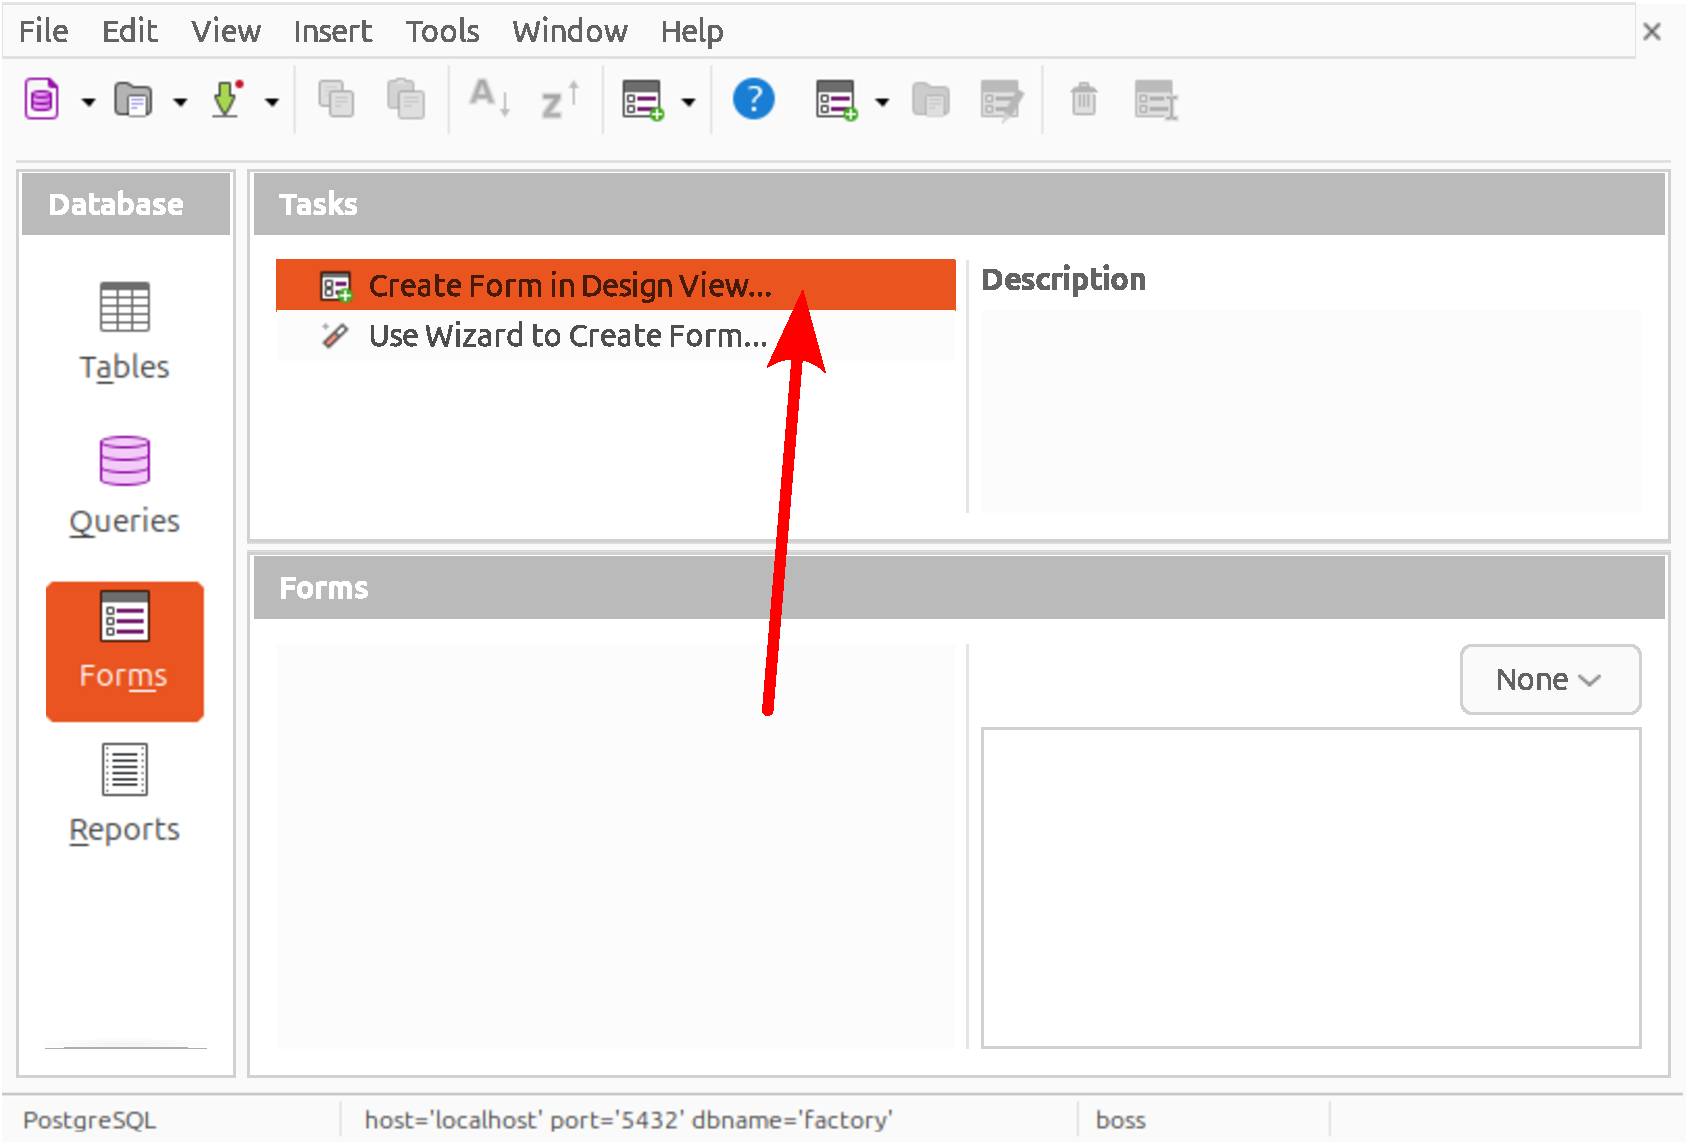
\includegraphics[width=0.49\linewidth]{\currentDir/factoryLibreOfficeBaseForms01createInDesignView}}}%
%
\floatSep%
%
\subfloat[][%
A new and empty form opens in the design view. %
We want to insert a tabular structure. %
The corresponding option is most likely hidden behind double-angle button~\libreOfficeBaseMore\ near the bottom on the pane on the left side.%
\label{fig:factoryLibreOfficeBaseForms02designView}%
]{\tightbox{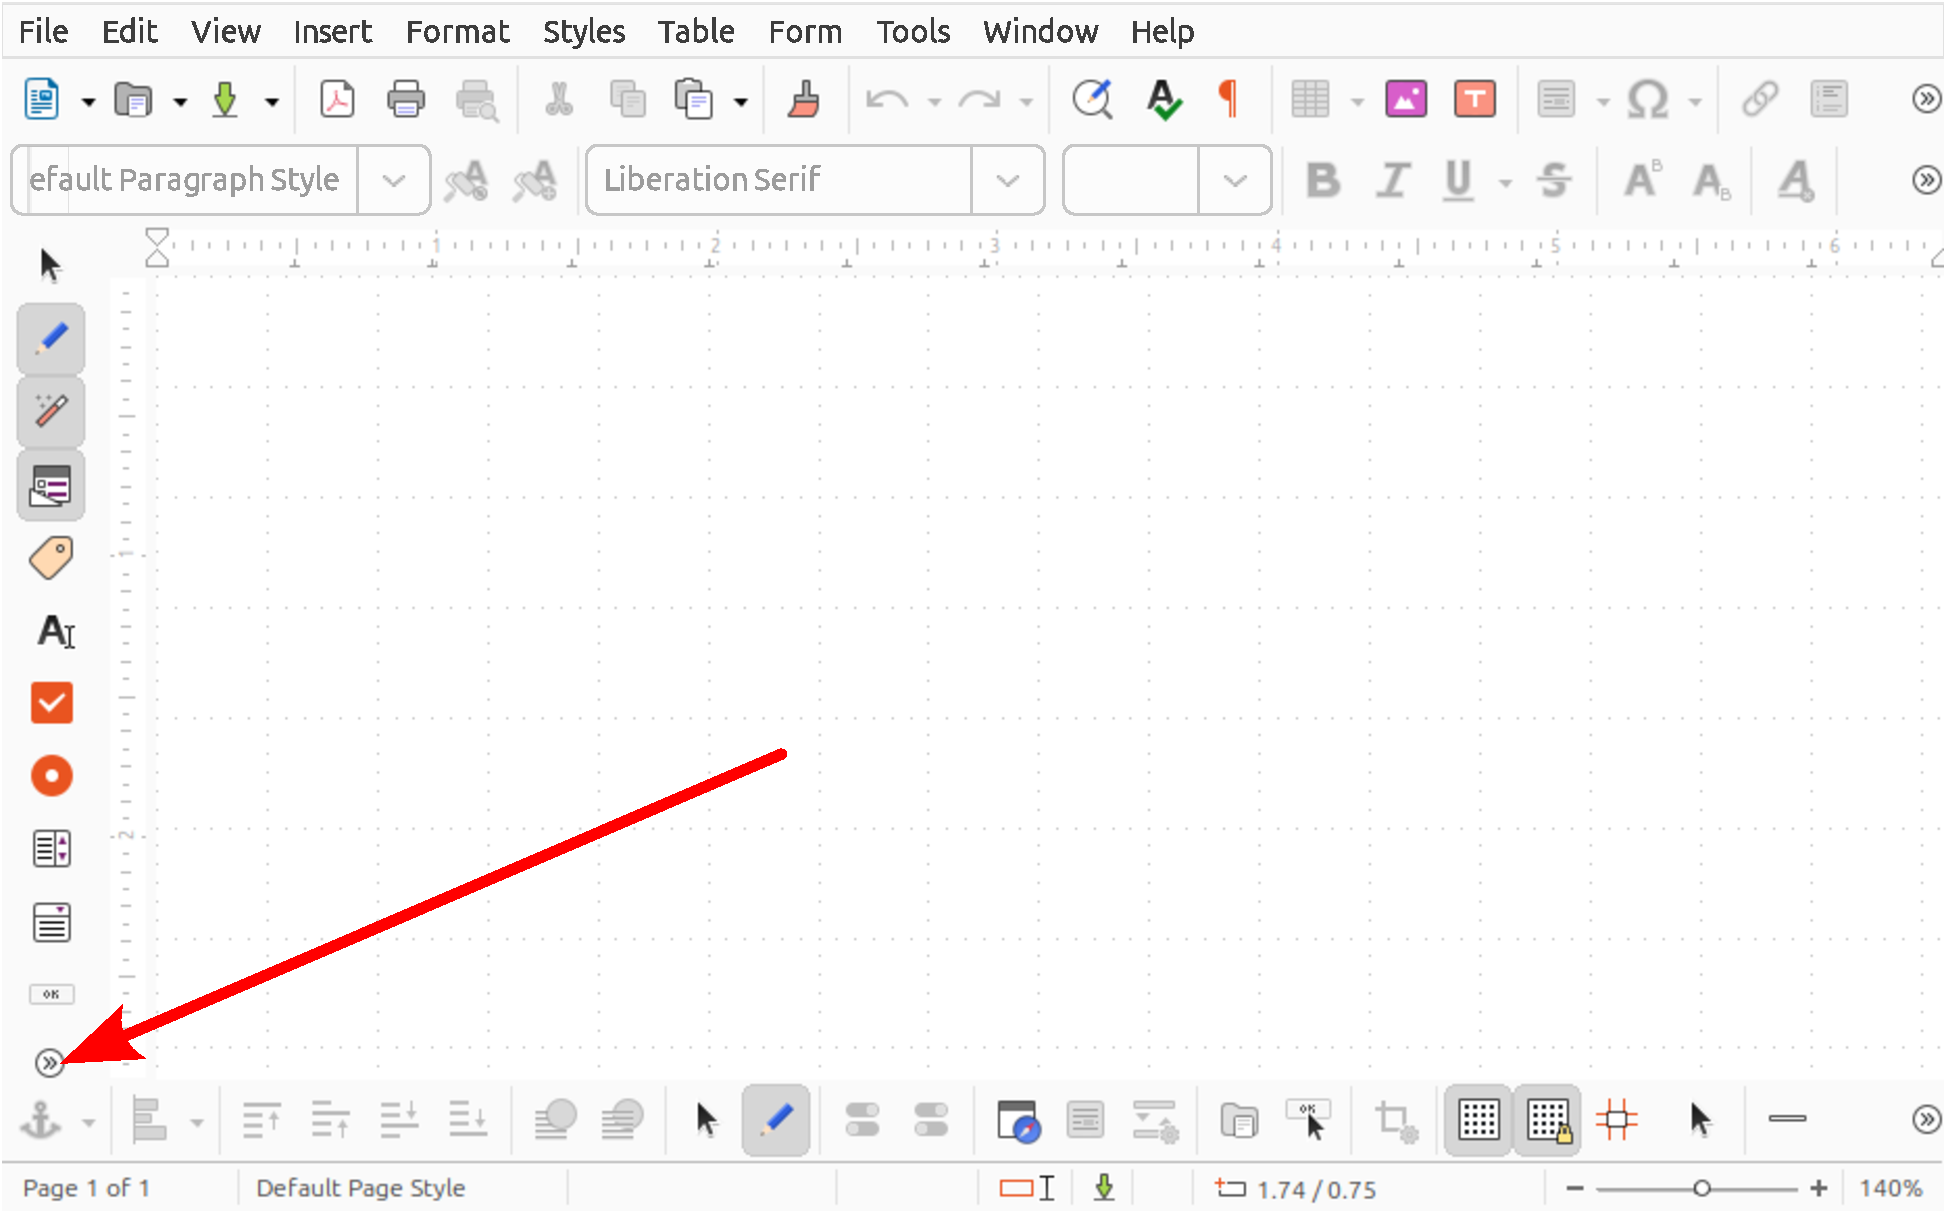
\includegraphics[width=0.49\linewidth]{\currentDir/factoryLibreOfficeBaseForms02designView}}}%
%
\floatRowSep%
%
\subfloat[][%
Click on the \menu{Table Control} button~\libreOfficeBaseTable.%
\label{fig:factoryLibreOfficeBaseForms03insertTable}%
]{\tightbox{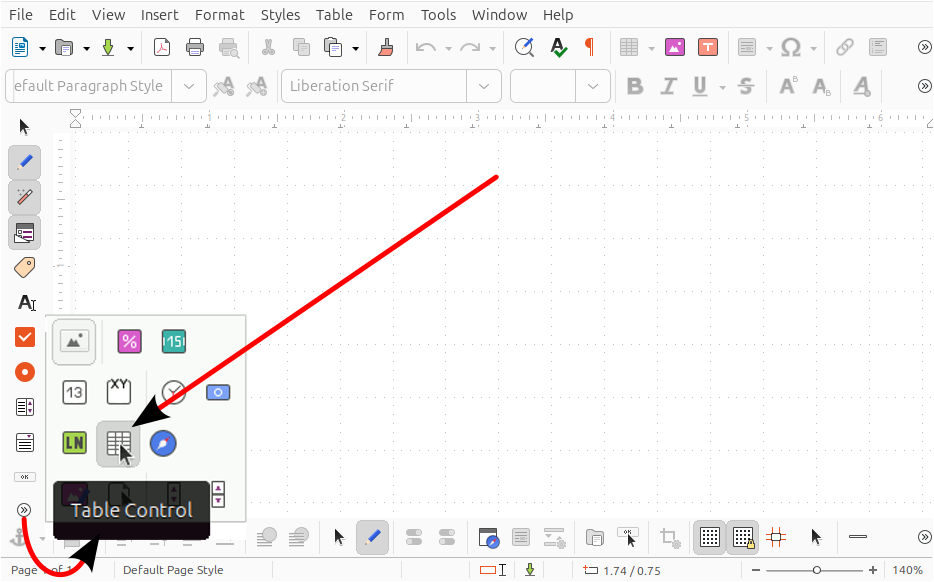
\includegraphics[width=0.49\linewidth]{\currentDir/factoryLibreOfficeBaseForms03insertTable}}}%
%
\floatSep%
%
\subfloat[][%
We click into the empty form body and drag the mouse to draw the table area. %
The we release the mouse.%
\label{fig:factoryLibreOfficeBaseForms04insertTable}%
]{\tightbox{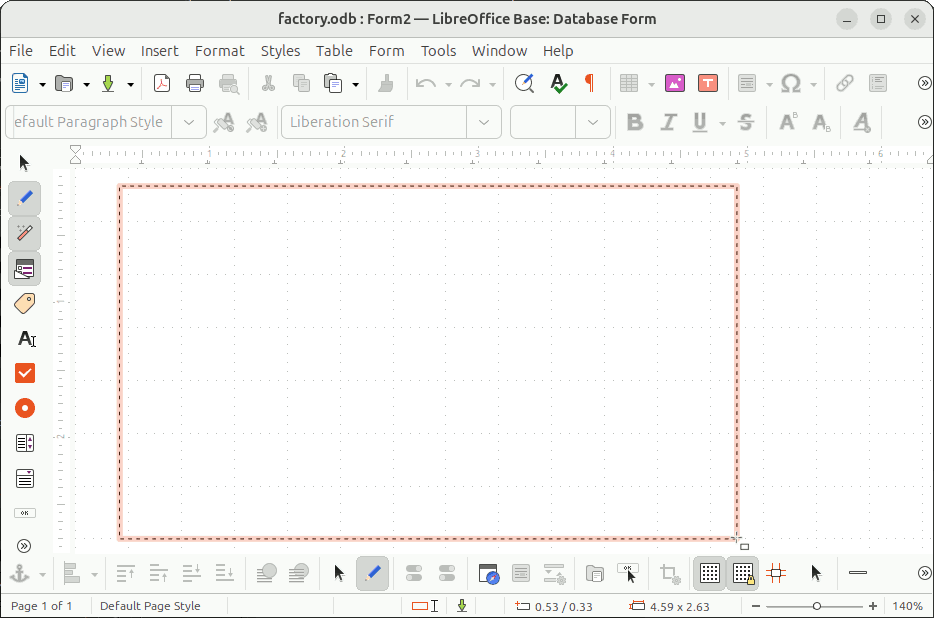
\includegraphics[width=0.49\linewidth]{\currentDir/factoryLibreOfficeBaseForms04insertTable}}}%
%
%
\floatRowSep%
%
\subfloat[][%
A dialog opens. %
It asks about the data we want to use in the table. %
We scroll down all the way in the view on the right side and select \inQuotes{public.demand.} %
We click \menu{Next}.%
\label{fig:factoryLibreOfficeBaseForms05selectSource}%
]{\tightbox{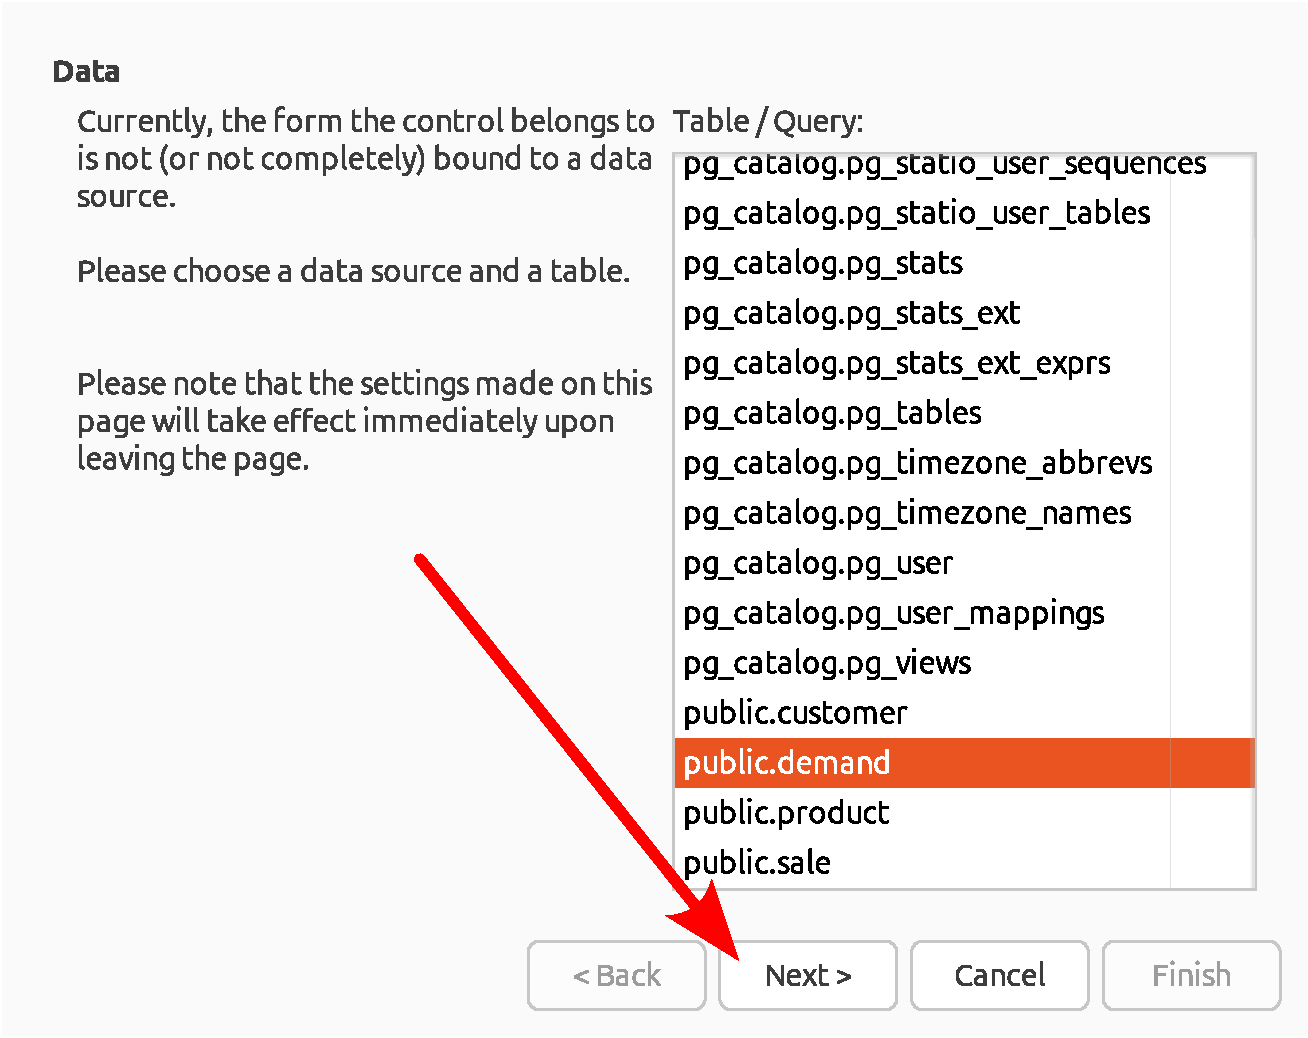
\includegraphics[width=0.49\linewidth]{\currentDir/factoryLibreOfficeBaseForms05selectSource}}}%
%
\floatSep%
%
\subfloat[][%
In the next dialog we can select columns to insert. %
We choose \sqlil{amount} and \sqlil{ordered}. %
We click \menu{Finish}.%
\label{fig:factoryLibreOfficeBaseForms06tableElements}%
]{\tightbox{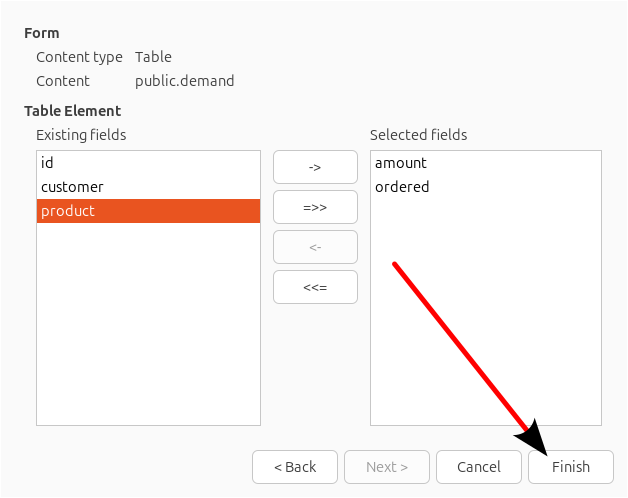
\includegraphics[width=0.49\linewidth]{\currentDir/factoryLibreOfficeBaseForms06tableElements}}}%
%
%
\caption{Creating a form for entering demand orders into our \db\ in \libreofficeBase.}%
\label{fig:factoryLibreOfficeBaseFormsA}%
%
\end{figure}%
%
\begin{figure}%
\ContinuedFloat%
\centering%
%
\subfloat[][%
The table is now inserted in draft form. %
We want to add more columns. %
Right-click at the left corner of the \sqlil{amount} column.%
\label{fig:factoryLibreOfficeBaseForms07table}%
]{\tightbox{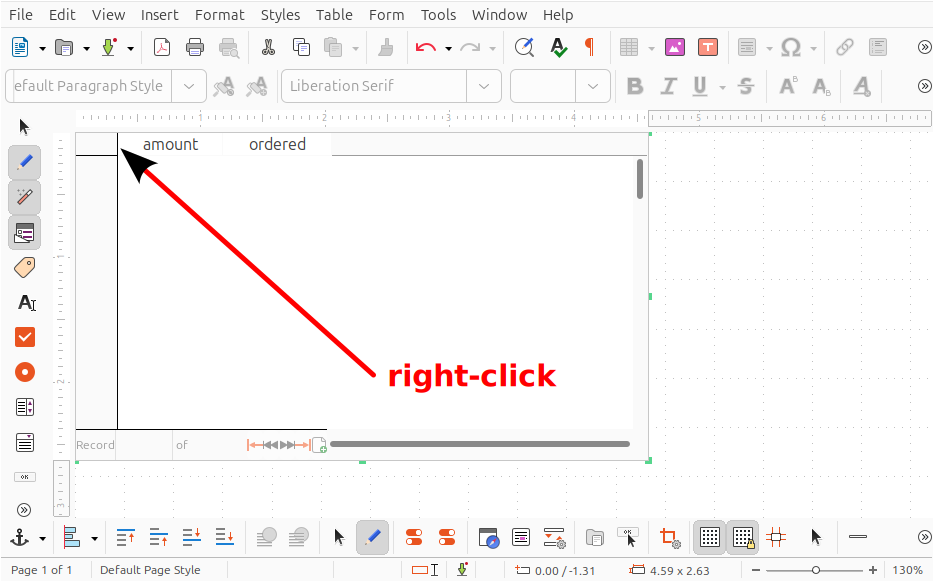
\includegraphics[width=0.49\linewidth]{\currentDir/factoryLibreOfficeBaseForms07table}}}%
%
\floatSep%
%
\subfloat[][%
In the menu that opens, click \menu{Insert Column} and then \menu{List Box}.%
\label{fig:factoryLibreOfficeBaseForms08addListColumn}%
]{\tightbox{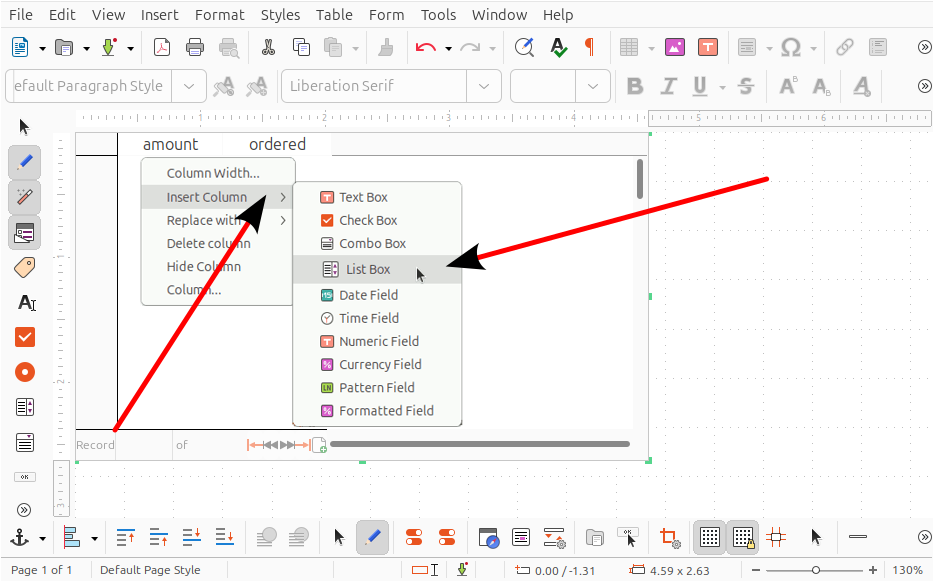
\includegraphics[width=0.49\linewidth]{\currentDir/factoryLibreOfficeBaseForms08addListColumn}}}%
%
\floatRowSep%
%
\subfloat[][%
A new column \inQuotes{List Box 1} has been added. %
We right-click on it.%
\label{fig:factoryLibreOfficeBaseForms09listColumnAdded}%
]{\tightbox{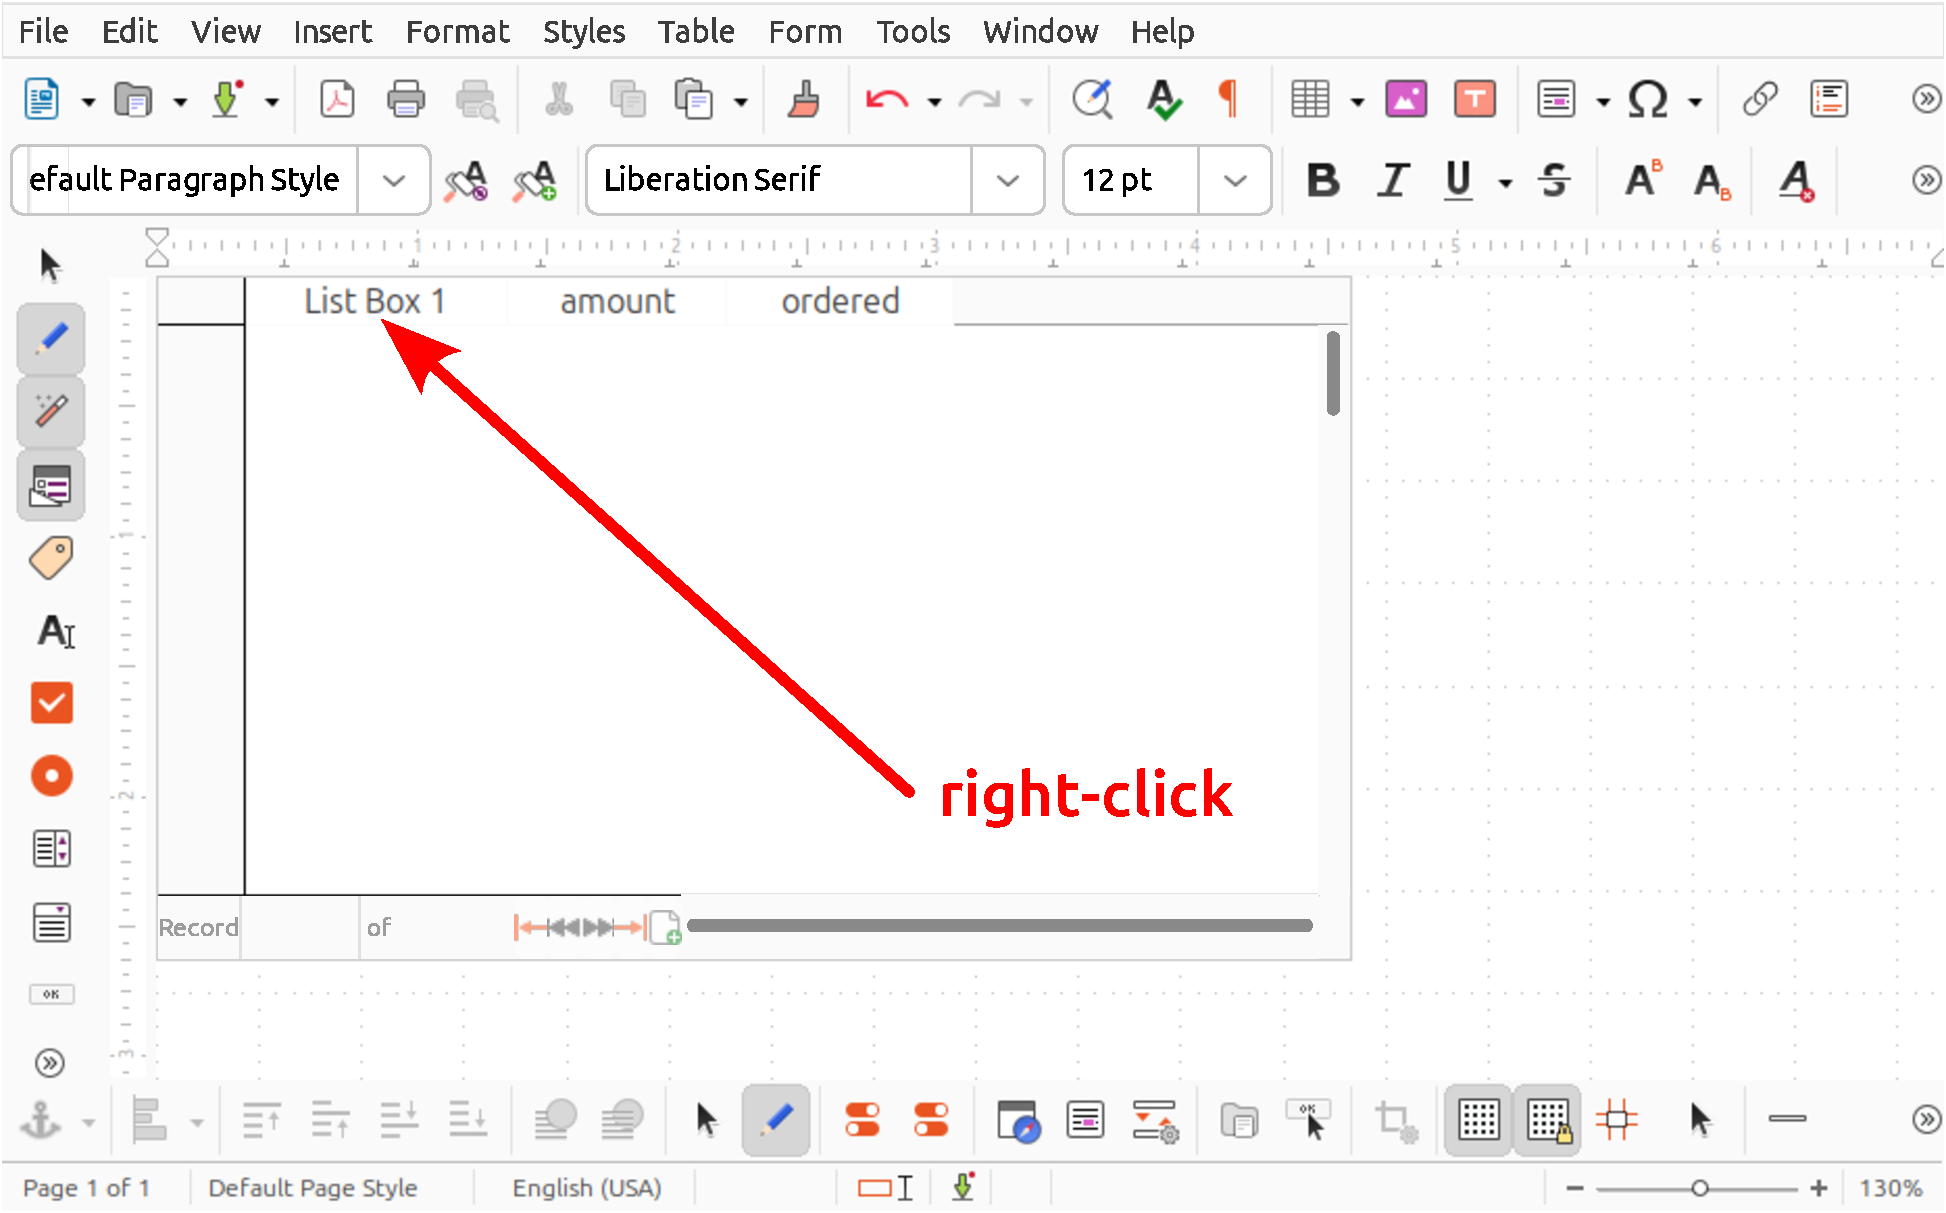
\includegraphics[width=0.49\linewidth]{\currentDir/factoryLibreOfficeBaseForms09listColumnAdded}}}%
%
\floatSep%
%
\subfloat[][%
In the menu that opens, click \menu{Column\dots}.%
\label{fig:factoryLibreOfficeBaseForms10editListColumn}%
]{\tightbox{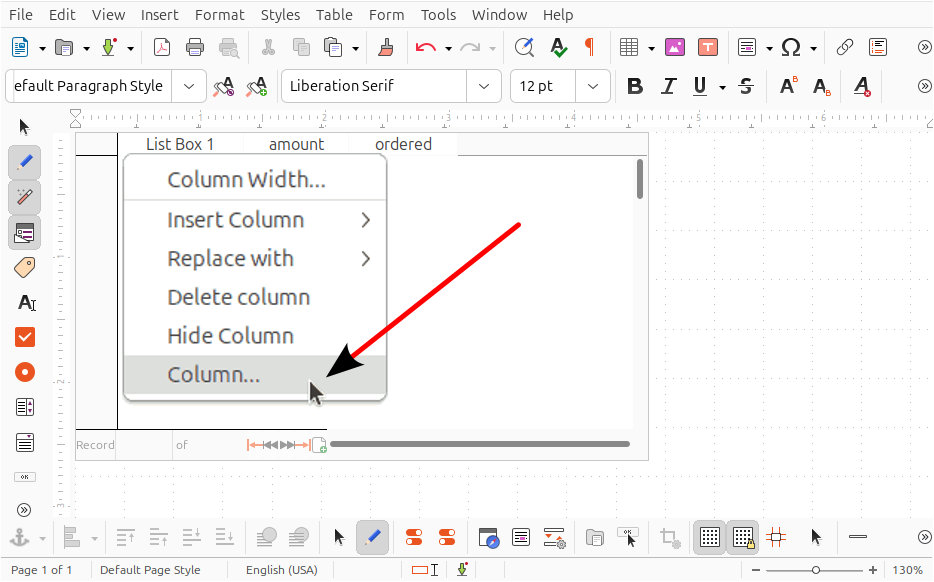
\includegraphics[width=0.49\linewidth]{\currentDir/factoryLibreOfficeBaseForms10editListColumn}}}%
%
\floatRowSep%
%
\subfloat[][%
First, we select the \menu{General} tab in the dialog that opens. %
We want to change the name and label of the new column.%
\label{fig:factoryLibreOfficeBaseForms11generalOld}%
]{\tightbox{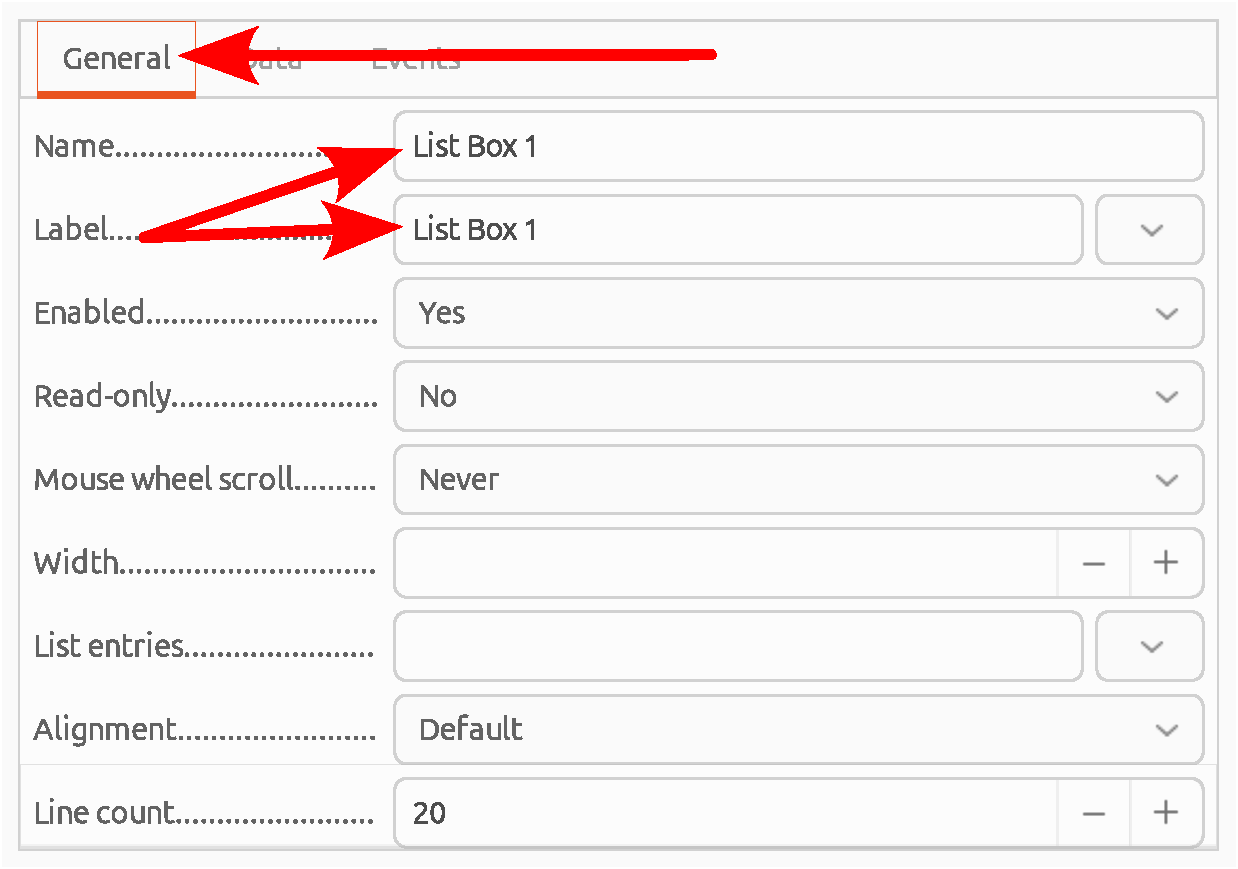
\includegraphics[width=0.49\linewidth]{\currentDir/factoryLibreOfficeBaseForms11generalOld}}}%
%
\floatSep%
%
\subfloat[][%
We change the label and the name of the column to \inQuotes{customer}. %
Then we click on the \menu{Data} pane.%
\label{fig:factoryLibreOfficeBaseForms12generalNew}%
]{\tightbox{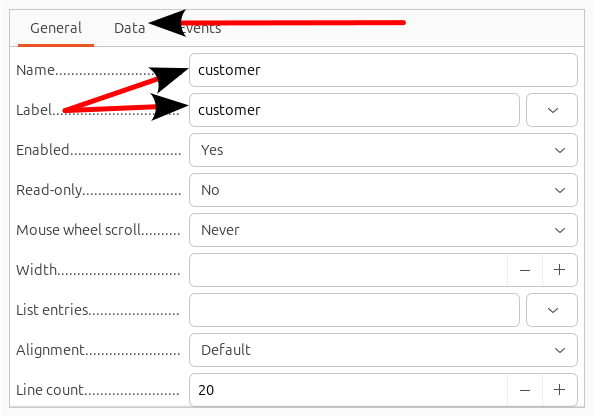
\includegraphics[width=0.49\linewidth]{\currentDir/factoryLibreOfficeBaseForms12generalNew}}}%
%
%
\caption{Creating a form for entering demand orders into our \db\ in \libreofficeBase~(Continued).}%
\label{fig:factoryLibreOfficeBaseFormsB}%
%
\end{figure}%
%
\begin{figure}%
\ContinuedFloat%
\centering%
%
\subfloat[][%
We first need to choose the column of our \sqlil{demand} table that should be set via this form field. %
We type in \sqlil{customer}.%
\label{fig:factoryLibreOfficeBaseForms13dataOld}%
]{\tightbox{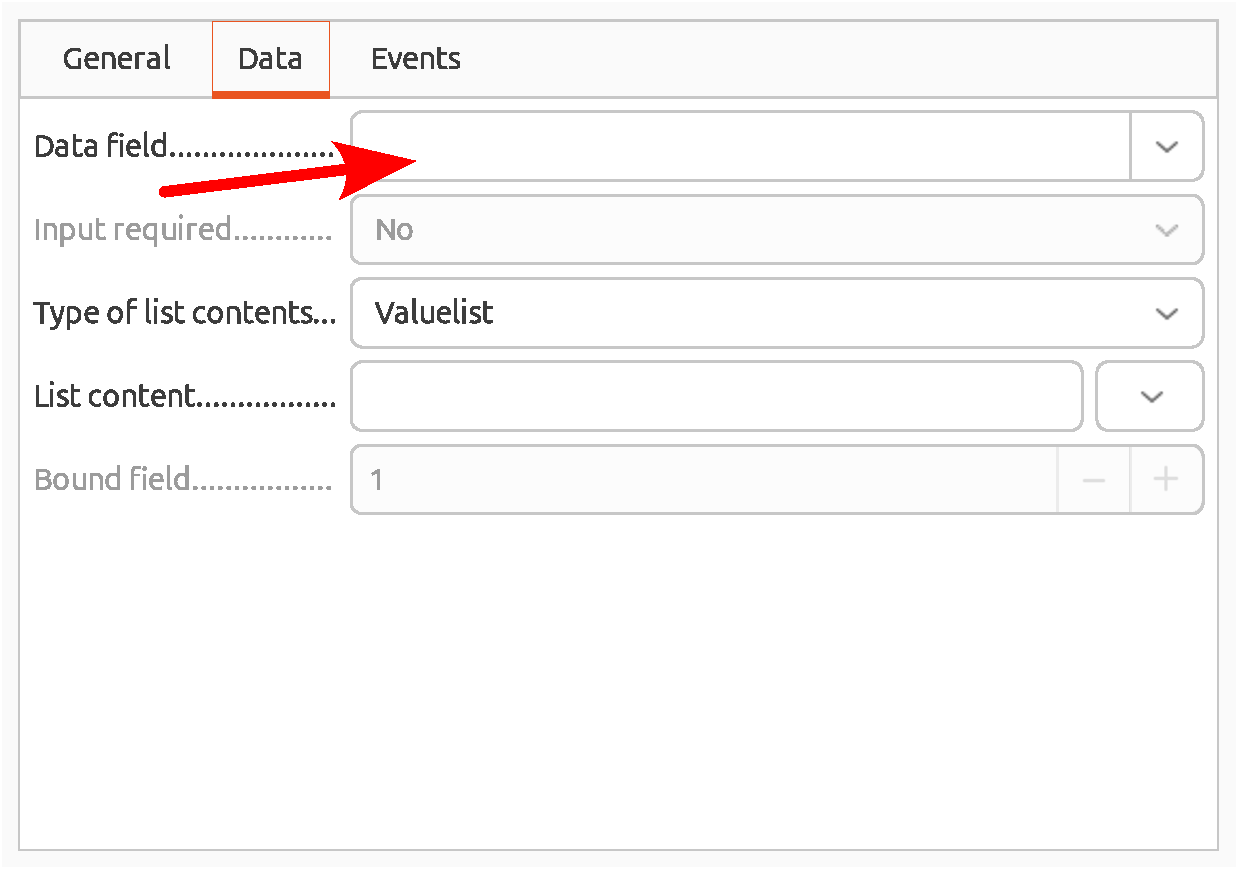
\includegraphics[width=0.49\linewidth]{\currentDir/factoryLibreOfficeBaseForms13dataOld}}}%
%
\floatSep%
%
\subfloat[][%
Next we want to change the \emph{Type of list contents} and \emph{Input Required}\dots%
\label{fig:factoryLibreOfficeBaseForms14dataCustomer}%
]{\tightbox{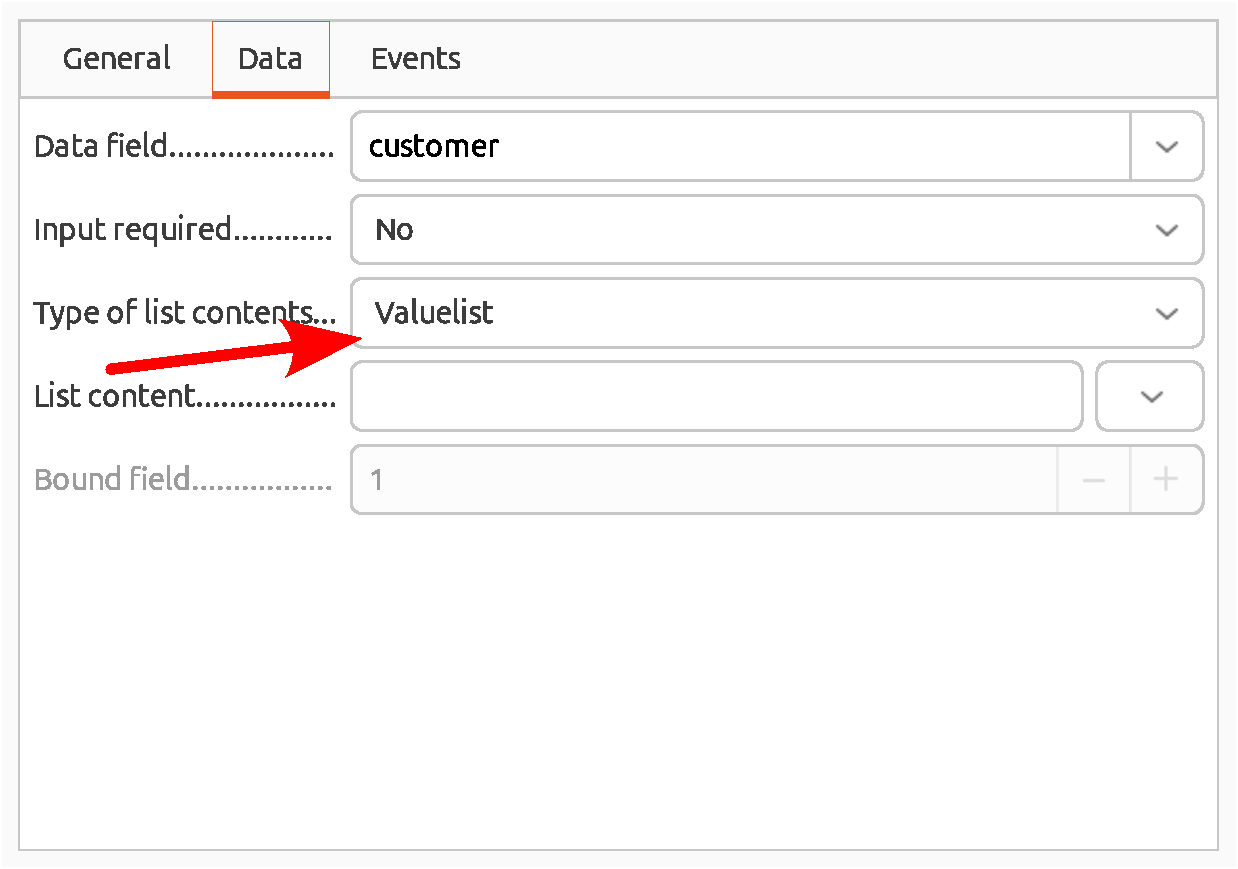
\includegraphics[width=0.49\linewidth]{\currentDir/factoryLibreOfficeBaseForms14dataCustomer}}}%
%
\floatRowSep%
%
\subfloat[][%
We change \emph{Input Required} to \menu{Yes}. %
We set \emph{Type of list contents} to \menu{Sql [Native]}. %
We click on the small wedge next to \emph{List content}.%
\label{fig:factoryLibreOfficeBaseForms15contentsSql}%
]{\tightbox{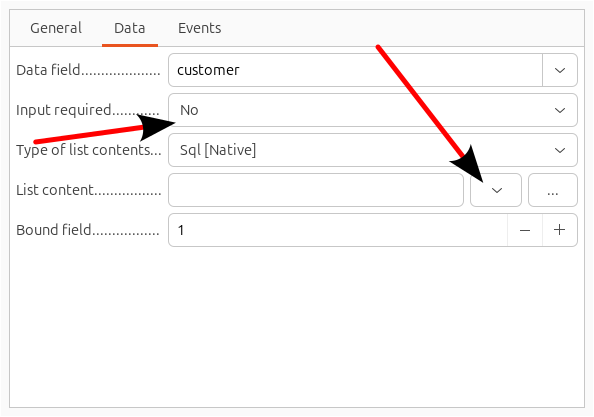
\includegraphics[width=0.49\linewidth]{\currentDir/factoryLibreOfficeBaseForms15contentsSql}}}%
%
\floatSep%
%
\subfloat[][%
We need to enter a \sql\ \sqlil{SELECT}\sqlIdx{SELECT{\idxdots}FROM} query that returns two values. %
We select both from table \sqlil{customer}, as follows: %
(1)~the one that should be displayed. %
We choose \sqlil{name || ', ' || phone}, i.e., a concatenation of the name and phone number string, separated by a comma. %
(2)~the one to be stored in the \sqlil{customer} field of the \sqlil{demand} table. %
We choose the customer \sqlil{id}.%
\label{fig:factoryLibreOfficeBaseForms16contentsQuery}%
]{\tightbox{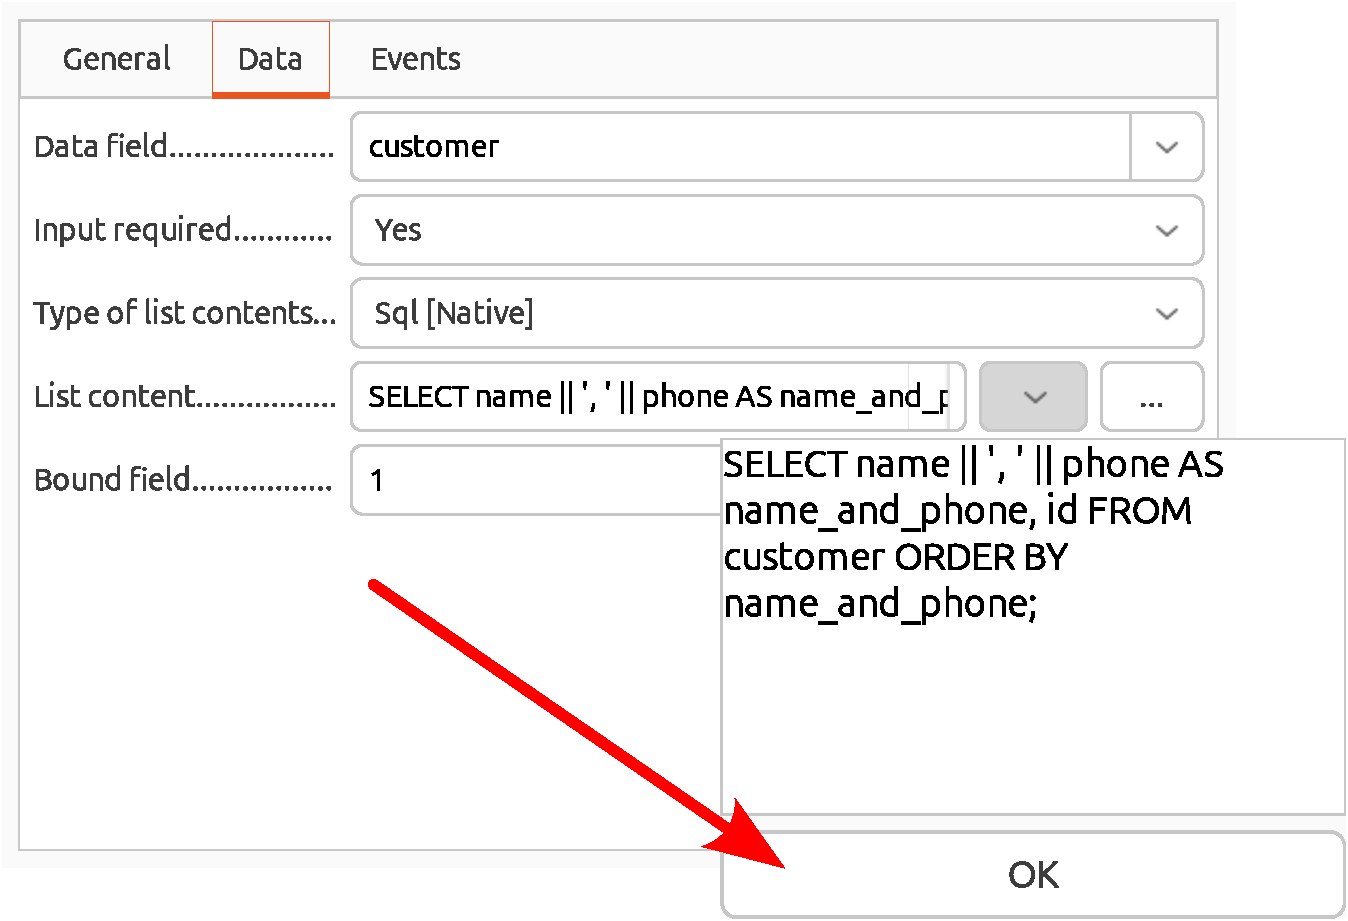
\includegraphics[width=0.49\linewidth]{\currentDir/factoryLibreOfficeBaseForms16contentsQuery}}}%
%
\floatRowSep%
%
\subfloat[][%
After we clicked \menu{OK} and closed the dialog, the name of the new column has changed to \sqlil{customer}. %
It appears to be a bit small for the information that it will contain, so we right-click on it\dots%
\label{fig:factoryLibreOfficeBaseForms17customerColAdded}%
]{\tightbox{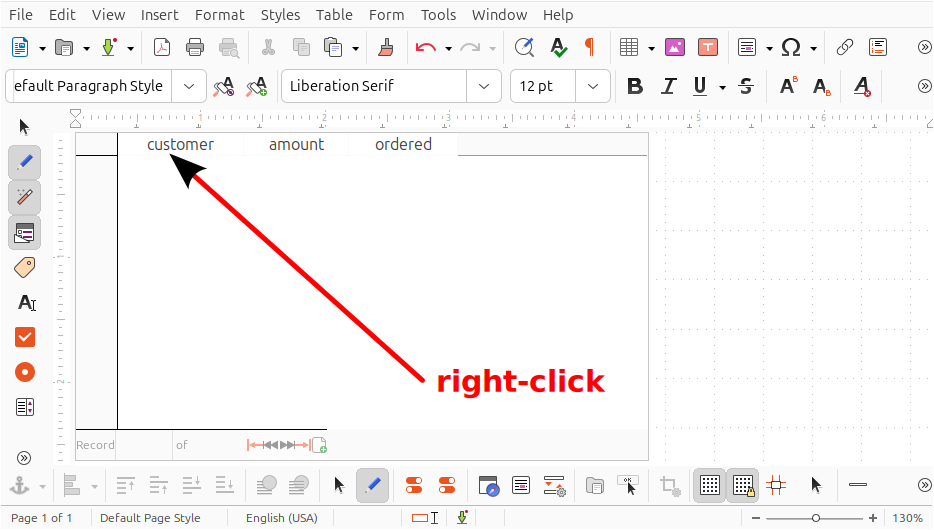
\includegraphics[width=0.49\linewidth]{\currentDir/factoryLibreOfficeBaseForms17customerColAdded}}}%
%
\floatSep%
%
\subfloat[][%
{\dots}and select \emph{Column width\dots} in the menu that pops up.%
\label{fig:factoryLibreOfficeBaseForms18customerSetColWidth}%
]{\tightbox{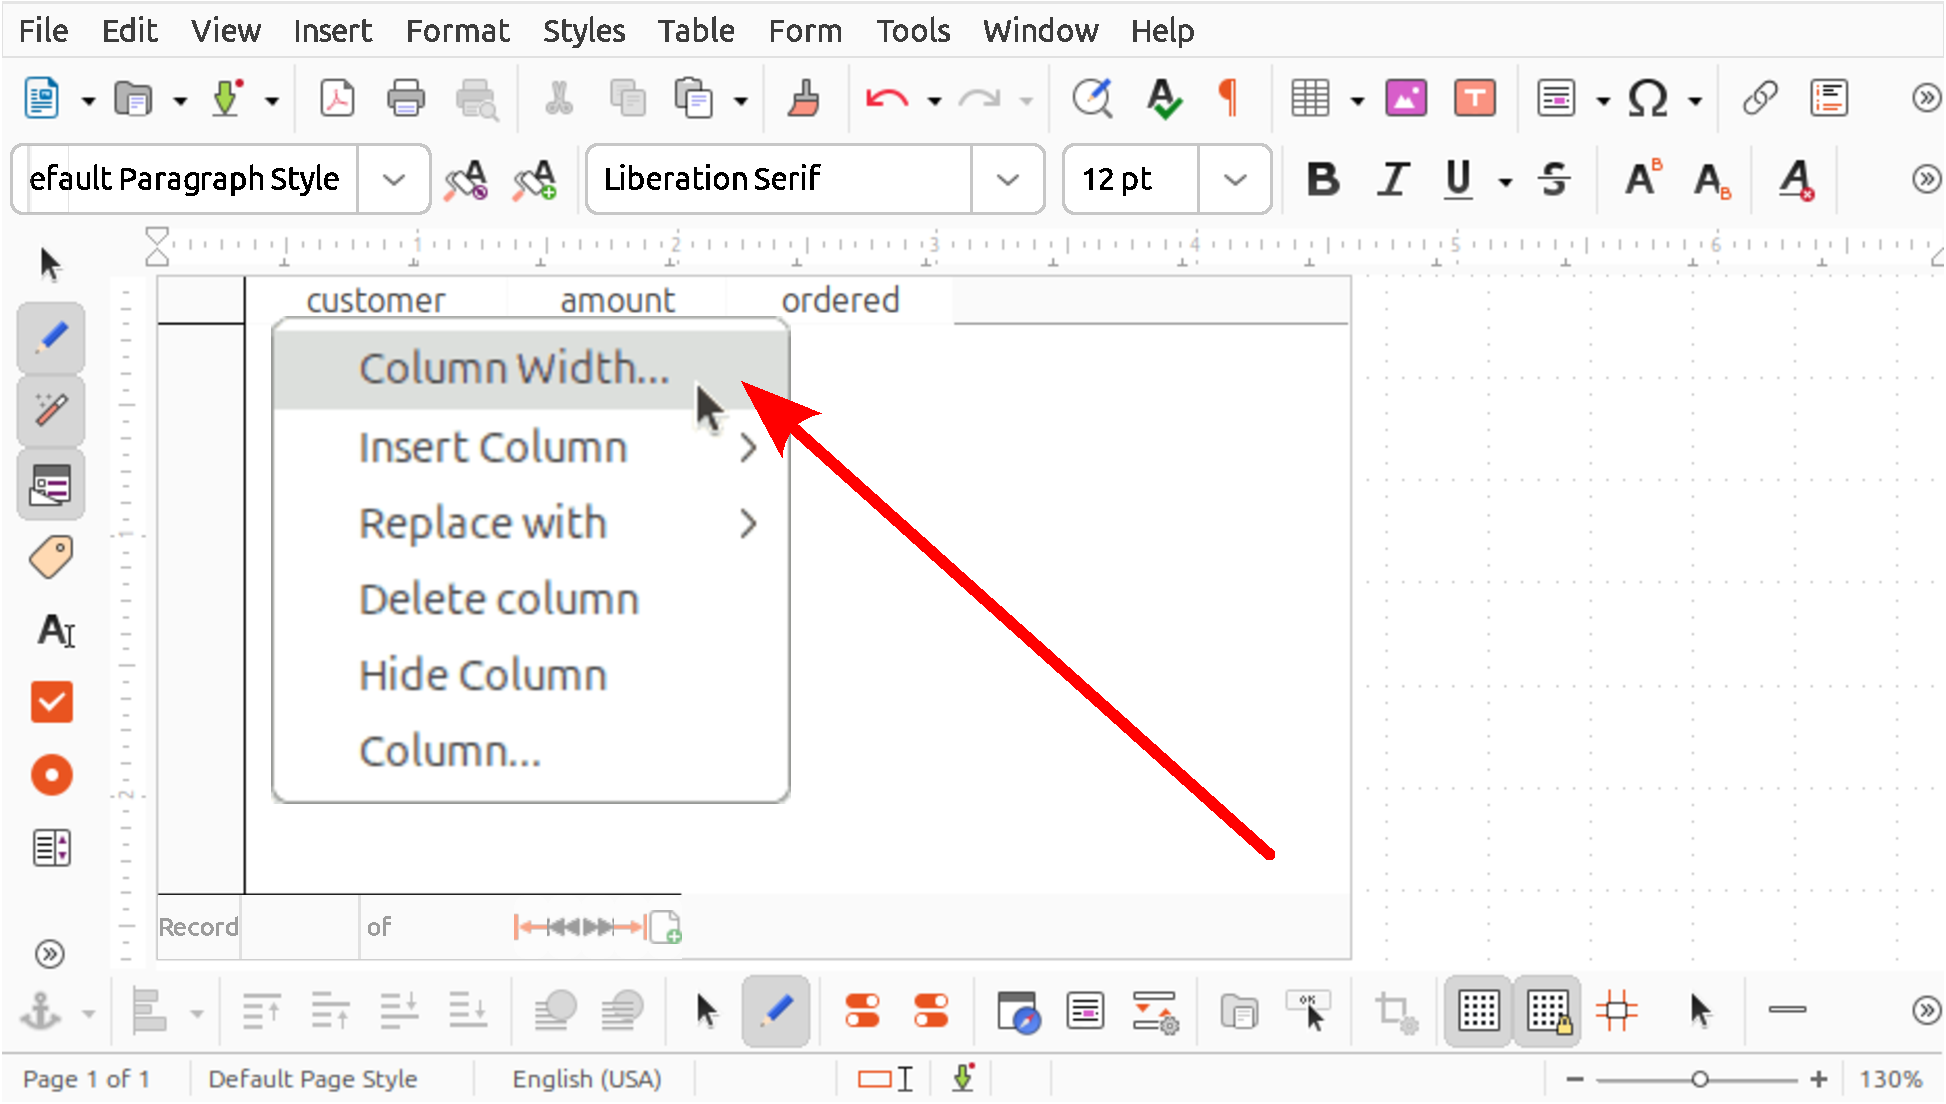
\includegraphics[width=0.49\linewidth]{\currentDir/factoryLibreOfficeBaseForms18customerSetColWidth}}}%
%
%
\caption{Creating a form for entering demand orders into our \db\ in \libreofficeBase~(Continued).}%
\label{fig:factoryLibreOfficeBaseFormsC}%
%
\end{figure}%
%
\begin{figure}%
\ContinuedFloat%
\centering%
%
\subfloat[][%
We write 4cm as \menu{Width} and click \menu{OK}.%
\label{fig:factoryLibreOfficeBaseForms19customerSetColWidth}%
]{\tightbox{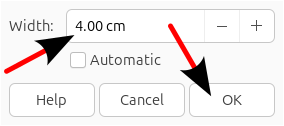
\includegraphics[width=0.49\linewidth]{\currentDir/factoryLibreOfficeBaseForms19customerSetColWidth}}}%
%
\floatSep%
%
\subfloat[][%
The column is wider now. %
We right-click between it and the \sqlil{amount} column.%
\label{fig:factoryLibreOfficeBaseForms20customerColConfigured}%
]{\tightbox{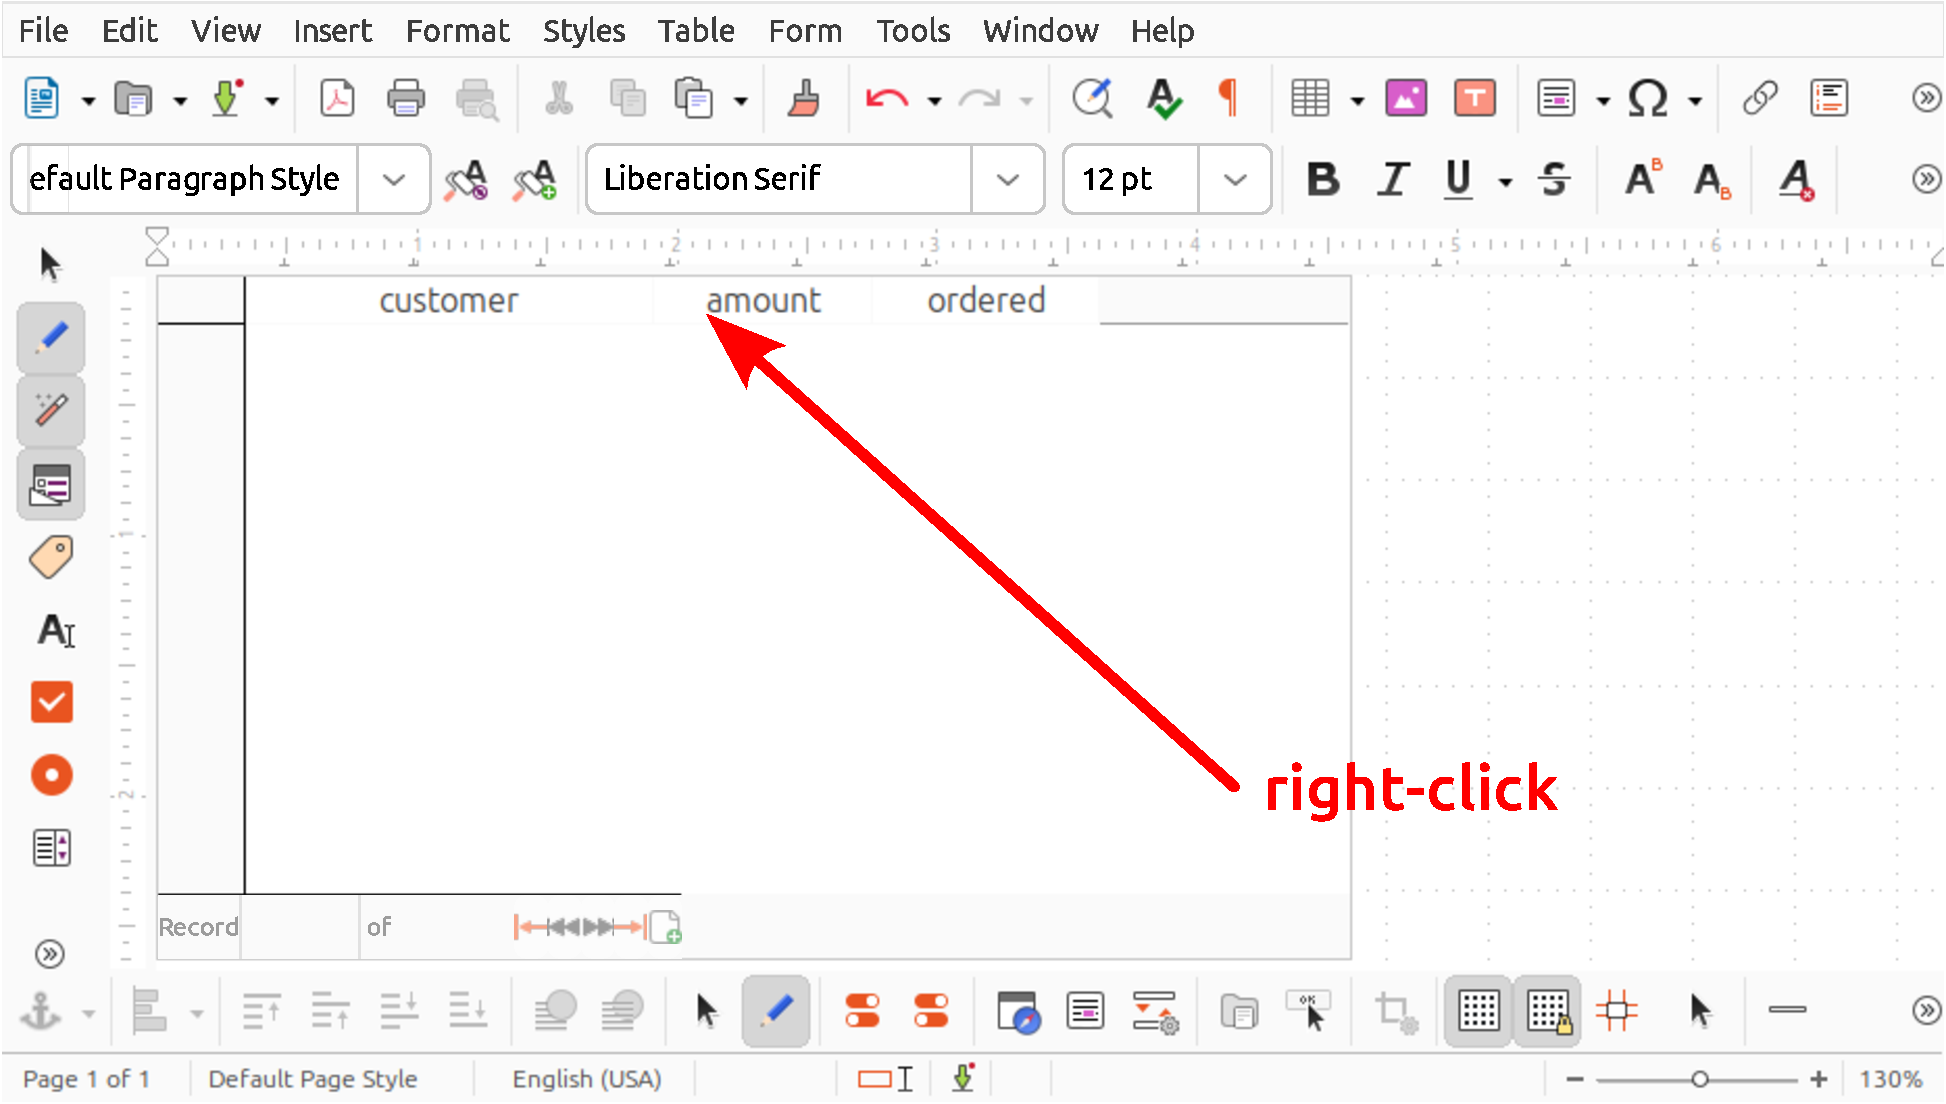
\includegraphics[width=0.49\linewidth]{\currentDir/factoryLibreOfficeBaseForms20customerColConfigured}}}%
%
\floatRowSep%
%
\subfloat[][%
In the menu that opens, we again click \menu{Insert Column} and then \menu{List Box}.%
\label{fig:factoryLibreOfficeBaseForms21insertColumn}%
]{\tightbox{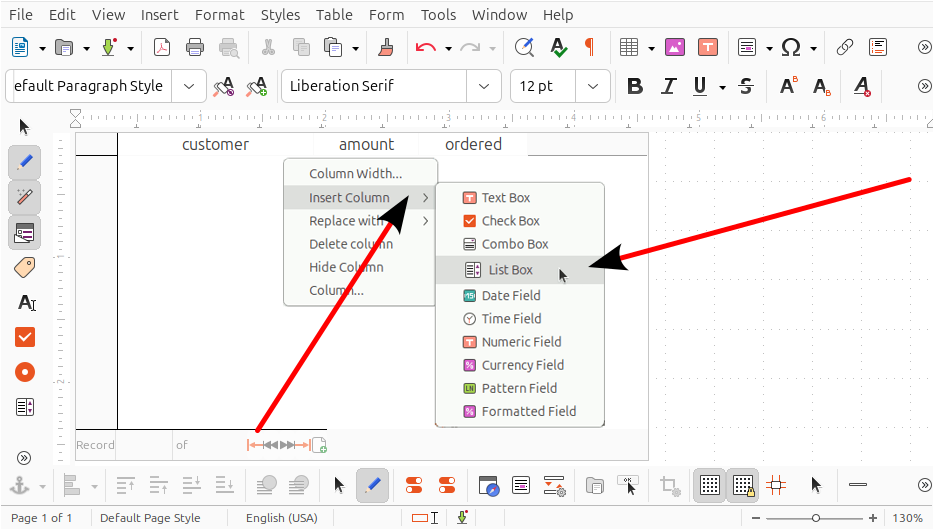
\includegraphics[width=0.49\linewidth]{\currentDir/factoryLibreOfficeBaseForms21insertColumn}}}%
%
\floatSep%
%
\subfloat[][%
A new \inQuotes{List Box 1} column appears. %
We right-click on it.%
\label{fig:factoryLibreOfficeBaseForms22columnInserted}%
]{\tightbox{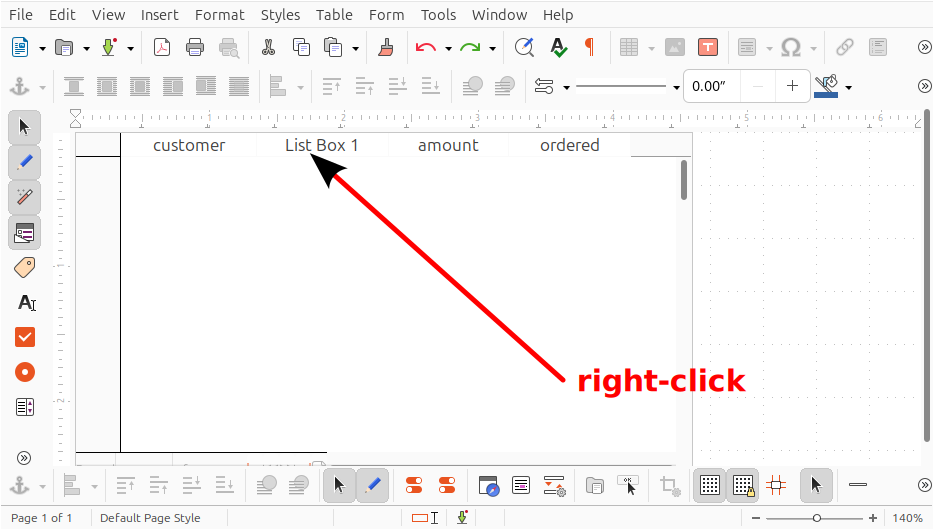
\includegraphics[width=0.49\linewidth]{\currentDir/factoryLibreOfficeBaseForms22columnInserted}}}%
%
\floatRowSep%
%
\subfloat[][%
In the menu that opens, we click on \menu{Column\dots}.%
\label{fig:factoryLibreOfficeBaseForms23columnEdit}%
]{\tightbox{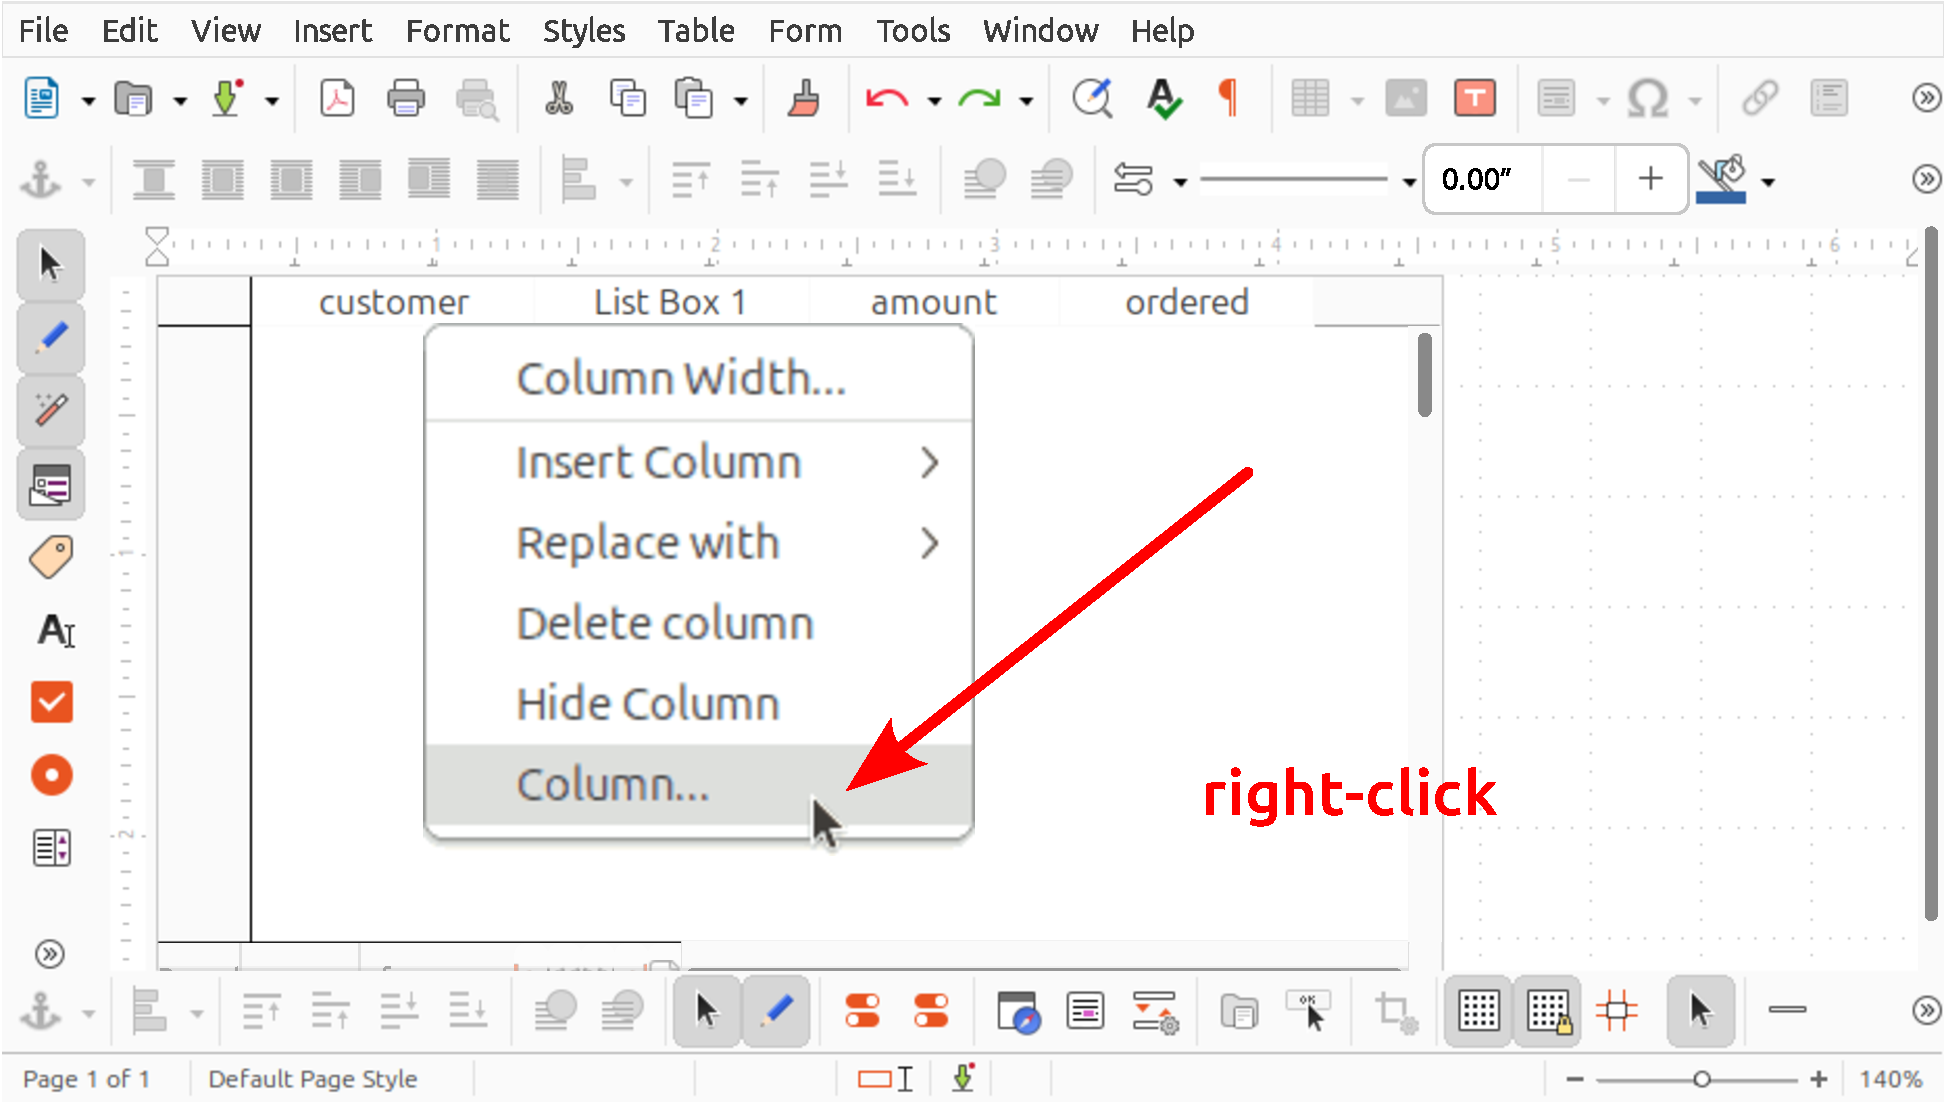
\includegraphics[width=0.49\linewidth]{\currentDir/factoryLibreOfficeBaseForms23columnEdit}}}%
%
\floatSep%
%
\subfloat[][%
In the \menu{General} properties pane, %
we set both the name and label to \sqlil{product} %
and the width to 1.57~inches.%
\label{fig:factoryLibreOfficeBaseForms24columnGeneralProperties}%
]{\tightbox{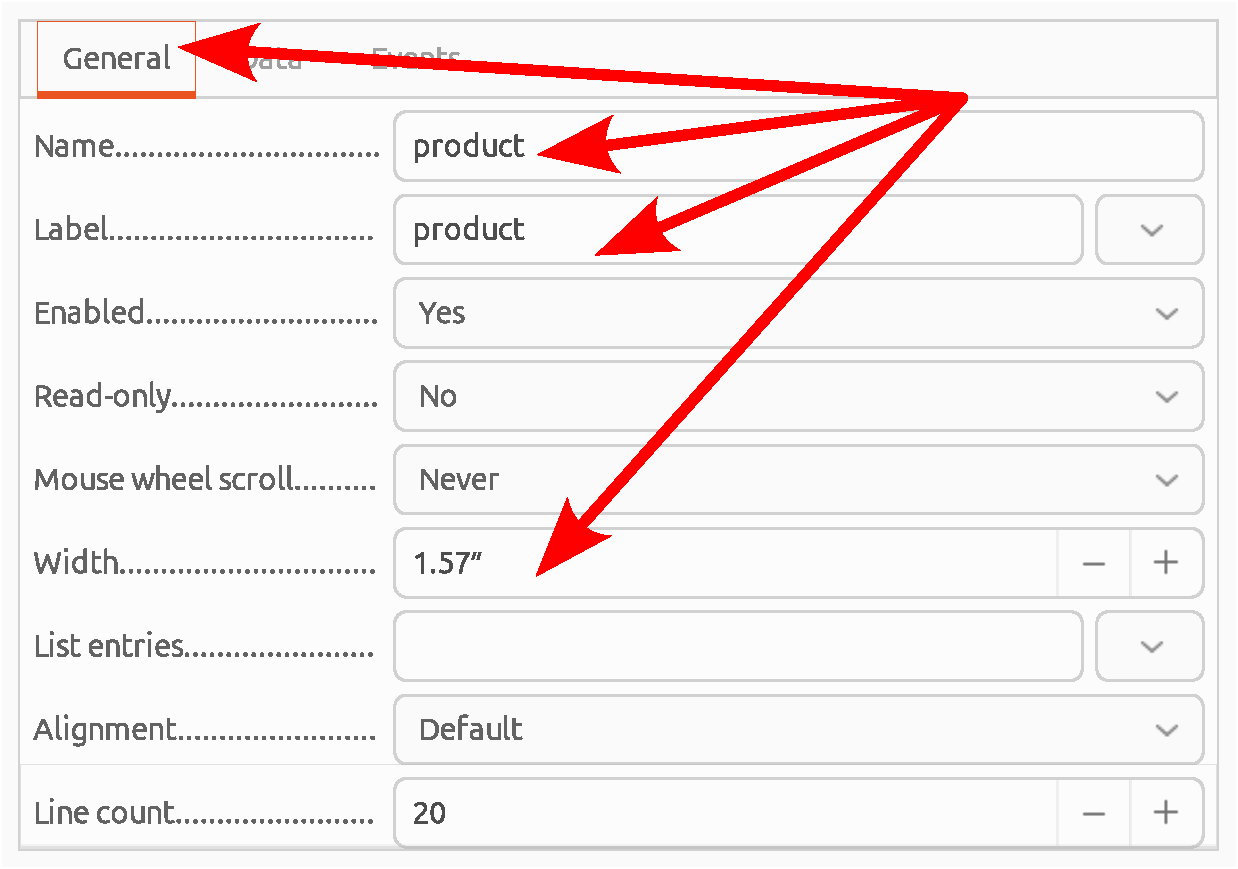
\includegraphics[width=0.49\linewidth]{\currentDir/factoryLibreOfficeBaseForms24columnGeneralProperties}}}%
%
%
\caption{Creating a form for entering demand orders into our \db\ in \libreofficeBase~(Continued).}%
\label{fig:factoryLibreOfficeBaseFormsD}%
%
\end{figure}%
%
\begin{figure}%
\ContinuedFloat%
\centering%
%
\subfloat[][%
In the \menu{Data} pane, we again enter a \sql\ query. %
This time, we select from table \sqlil{product}. %
The \sqlil{name} column should be displayed to the user, %
while the \sqlil{id} column should be stored in the form.%
\label{fig:factoryLibreOfficeBaseForms25columnSQL}%
]{\tightbox{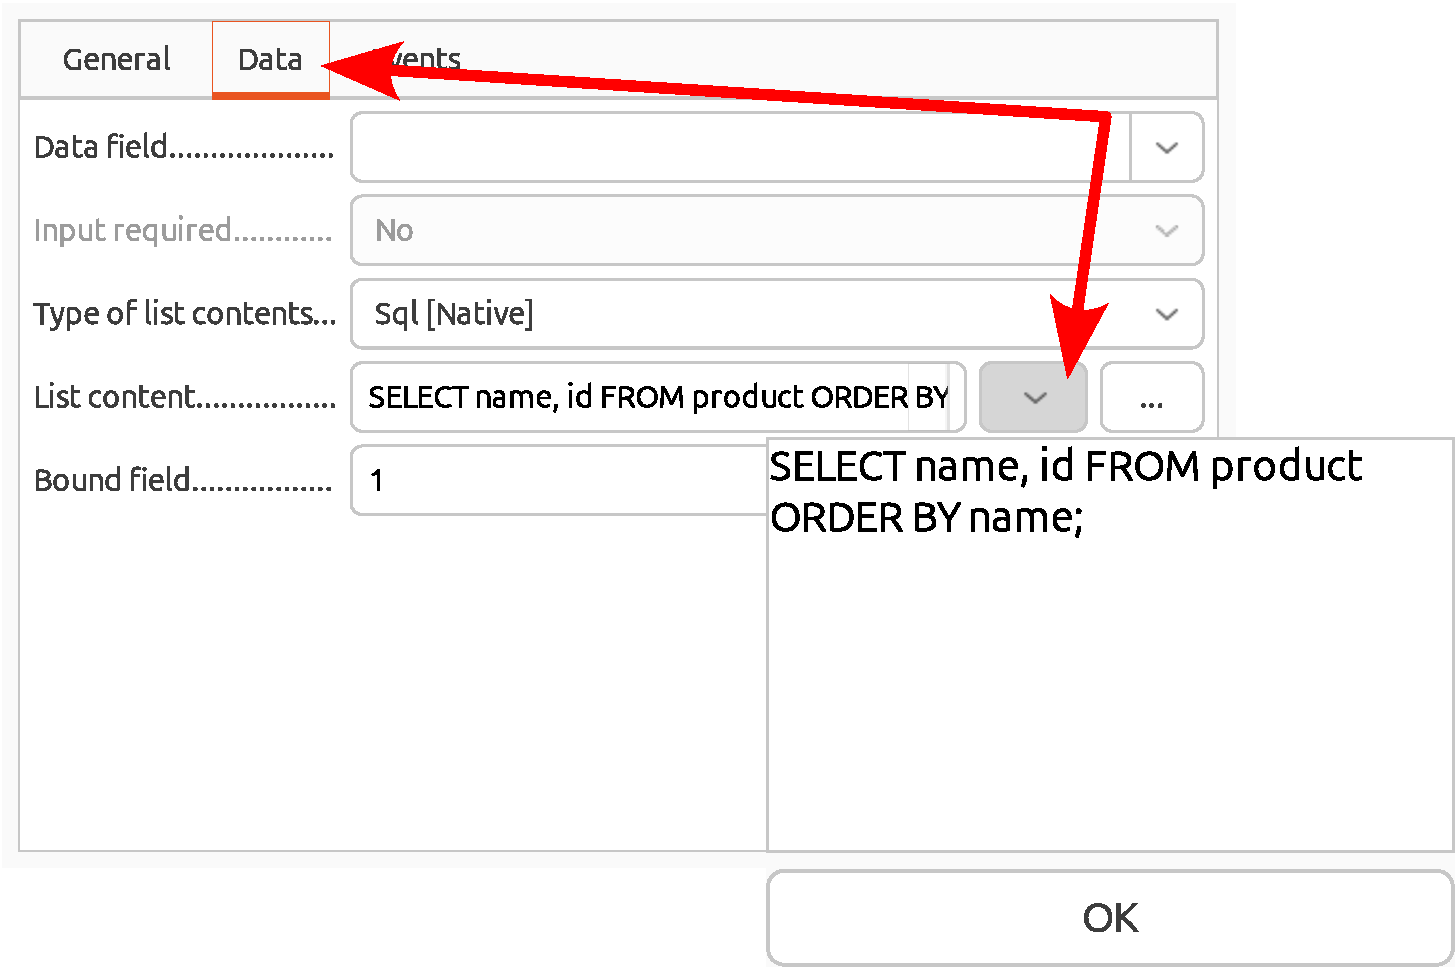
\includegraphics[width=0.49\linewidth]{\currentDir/factoryLibreOfficeBaseForms25columnSQL}}}%
%
\floatSep%
%
\subfloat[][%
The \sqlil{id} from the selected \sqlil{product} should be stored in the \sqlil{product} field of the \sqlil{demand} record. %
Therefore, we select \sqlil{product} as \emph{Data field\dots}%
\label{fig:factoryLibreOfficeBaseForms26columnData}%
]{\tightbox{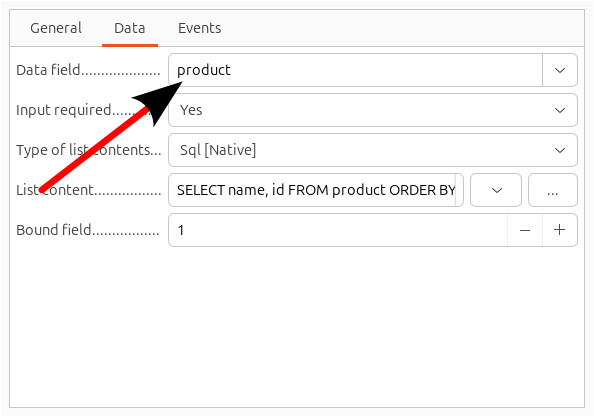
\includegraphics[width=0.49\linewidth]{\currentDir/factoryLibreOfficeBaseForms26columnData}}}%
%
\floatRowSep%
%
\subfloat[][%
We close the dialog. %
The form design is now finished. %
We unselect the pencil symbol~\libreOfficeBaseDesignMode\ in the bottom bar.%
\label{fig:factoryLibreOfficeBaseForms27formDesigned}%
]{\tightbox{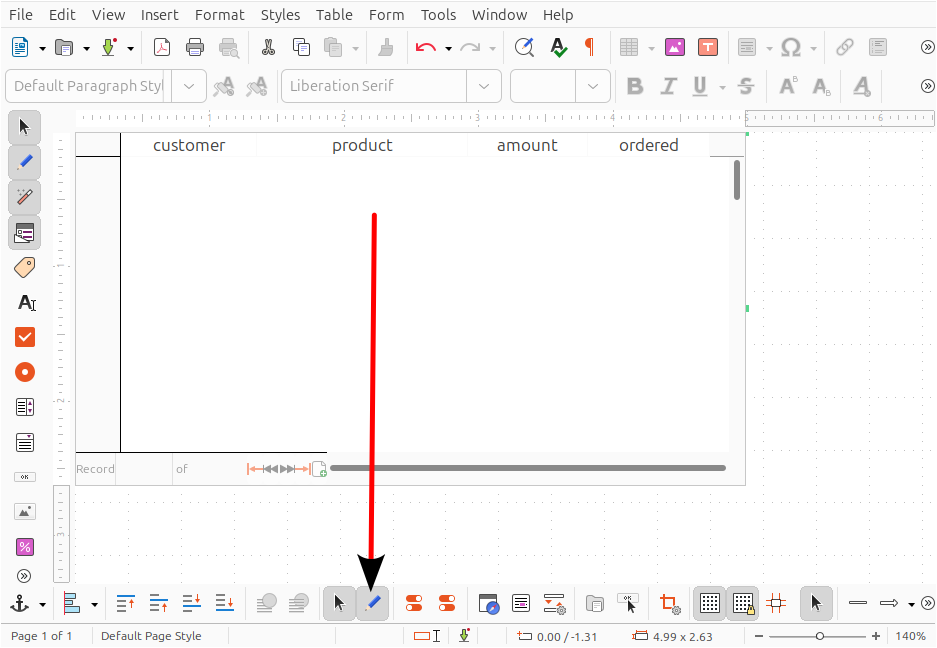
\includegraphics[width=0.49\linewidth]{\currentDir/factoryLibreOfficeBaseForms27formDesigned}}}%
%
\floatSep%
%
\subfloat[][%
This opens our form. %
It now displays the data to us in a form similar to the \sqlil{sale} view.%
\label{fig:factoryLibreOfficeBaseForms28formOpen}%
]{\tightbox{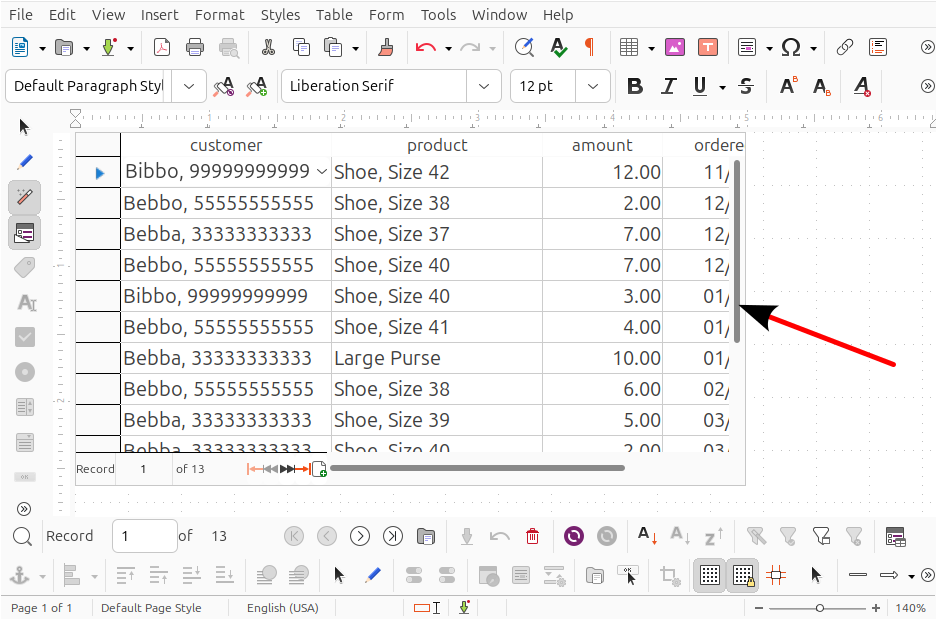
\includegraphics[width=0.49\linewidth]{\currentDir/factoryLibreOfficeBaseForms28formOpen}}}%
%
\floatRowSep%
%
\subfloat[][%
However, it is a \emph{form}, not a \emph{view}. %
We can edit the data and insert new data. %
We scroll down to the empty row at the very bottom. %
We click on the small wedge symbol in the \sqlil{customer} column.%
\label{fig:factoryLibreOfficeBaseForms29formUse}%
]{\tightbox{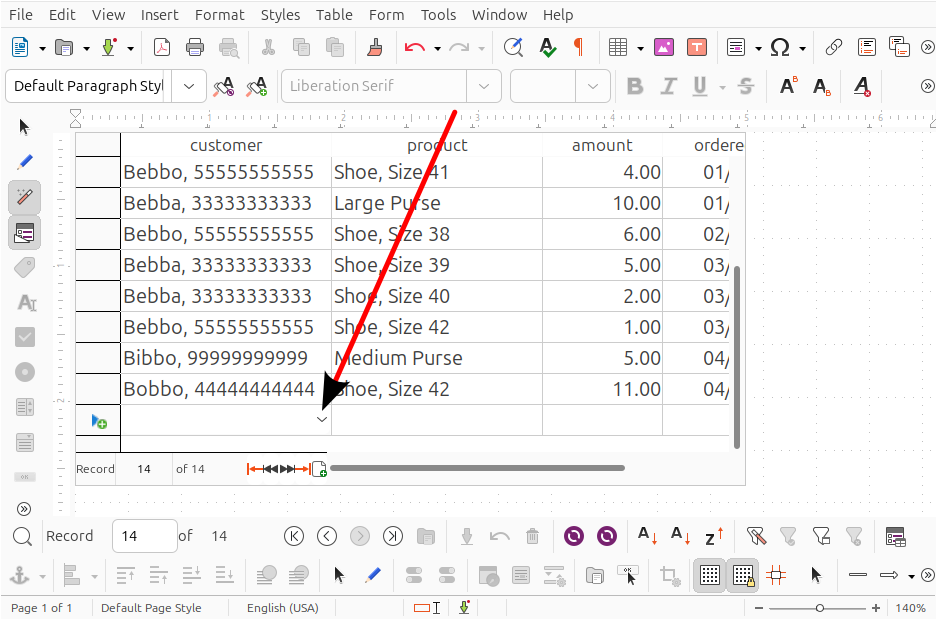
\includegraphics[width=0.49\linewidth]{\currentDir/factoryLibreOfficeBaseForms29formUse}}}%
%
\floatSep%
%
\subfloat[][%
A drop-down list opens from which we can select the customer in \emph{clearly readable form.} %
We choose Mr.~Bibbo.%
\label{fig:factoryLibreOfficeBaseForms30formUseCustomer}%
]{\tightbox{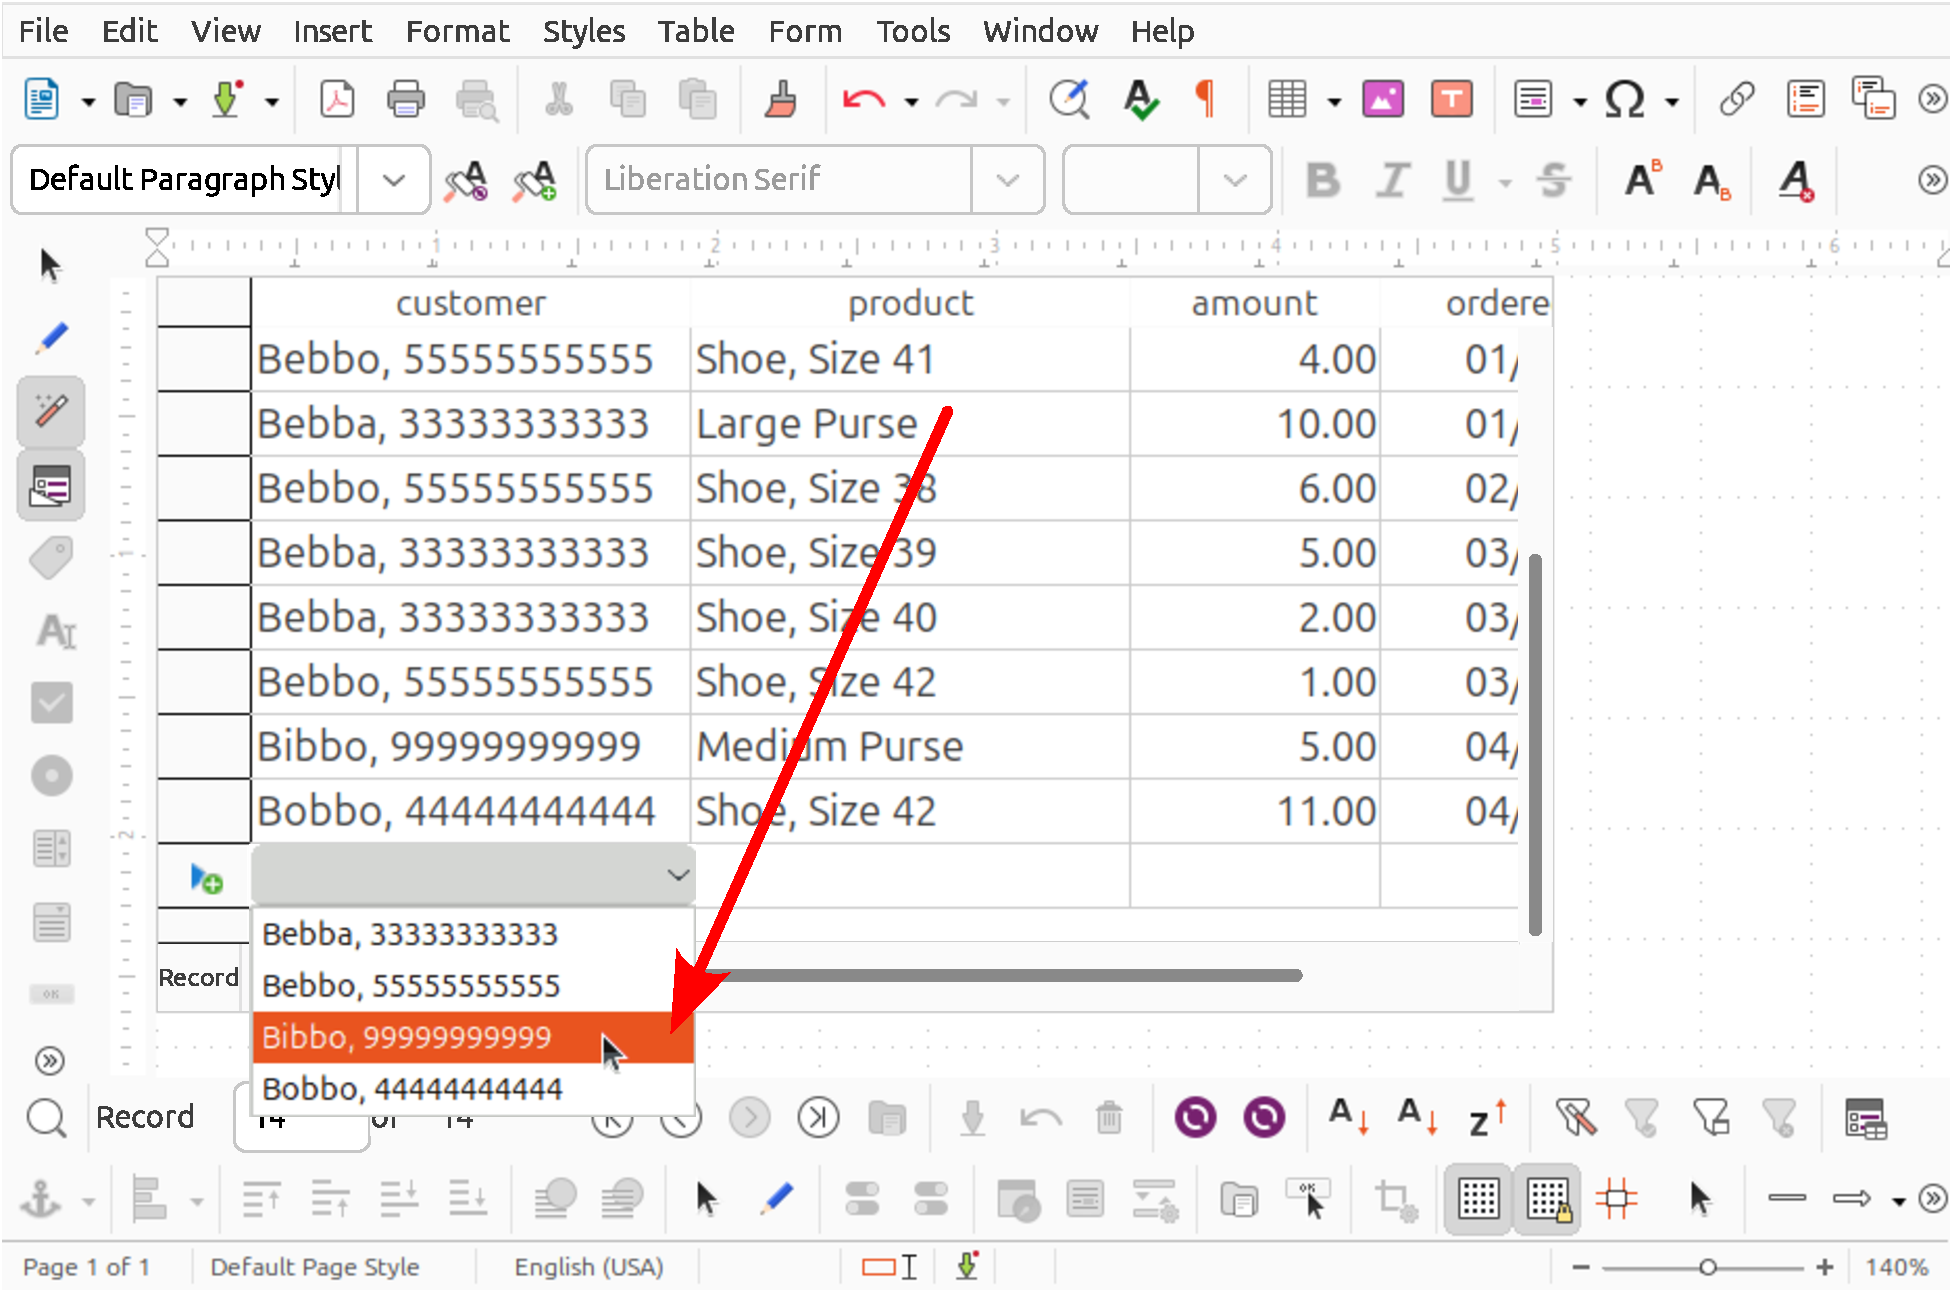
\includegraphics[width=0.49\linewidth]{\currentDir/factoryLibreOfficeBaseForms30formUseCustomer}}}%
%
%
\caption{Creating a form for entering demand orders into our \db\ in \libreofficeBase~(Continued).}%
\label{fig:factoryLibreOfficeBaseFormsE}%
%
\end{figure}%
%
\begin{figure}%
\ContinuedFloat%
\centering%
%
\subfloat[][%
We now click on the small wedge in the \sqlil{product} column.%
\label{fig:factoryLibreOfficeBaseForms31formUseCustomerDone}%
]{\tightbox{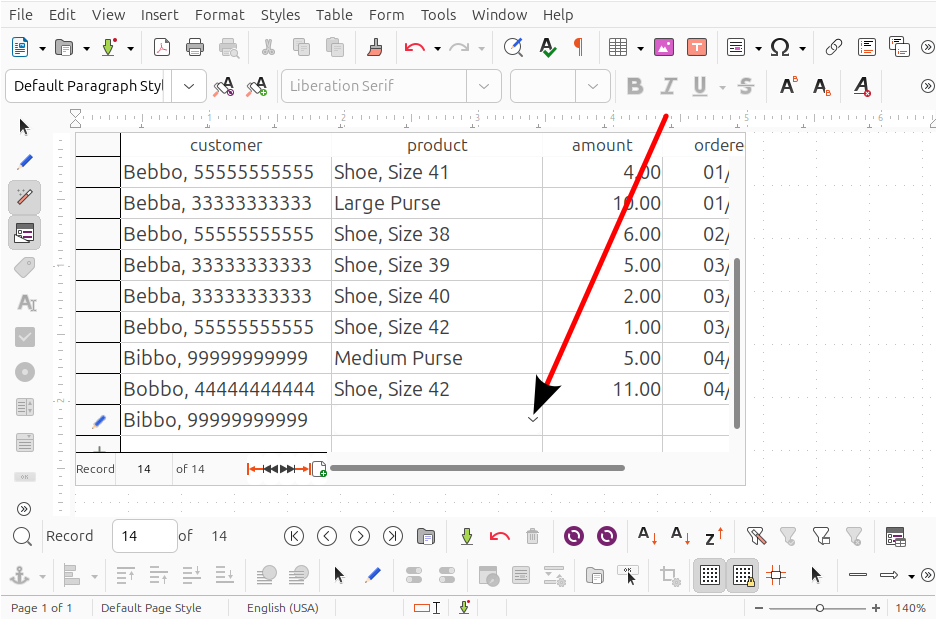
\includegraphics[width=0.49\linewidth]{\currentDir/factoryLibreOfficeBaseForms31formUseCustomerDone}}}%
%
\floatSep%
%
\subfloat[][%
In the drop-down list that opens, we select \inQuotes{Shoe, Size 39}.%
\label{fig:factoryLibreOfficeBaseForms32formUseProduct}%
]{\tightbox{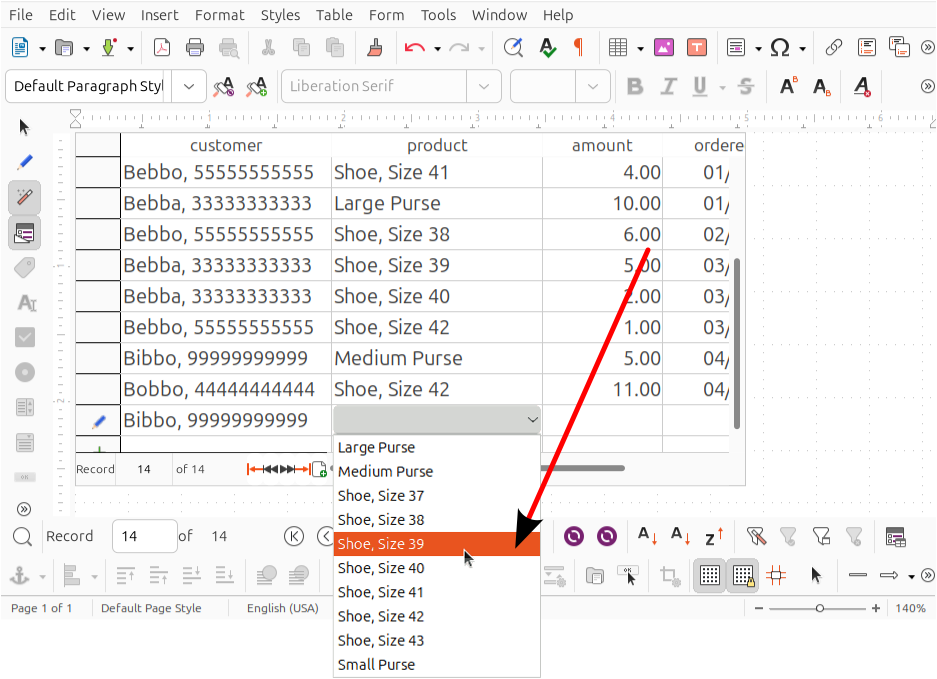
\includegraphics[width=0.49\linewidth]{\currentDir/factoryLibreOfficeBaseForms32formUseProduct}}}%
%
\floatRowSep%
%
\subfloat[][%
We can now enter the amount.%
\label{fig:factoryLibreOfficeBaseForms33formUseProductDone}%
]{\tightbox{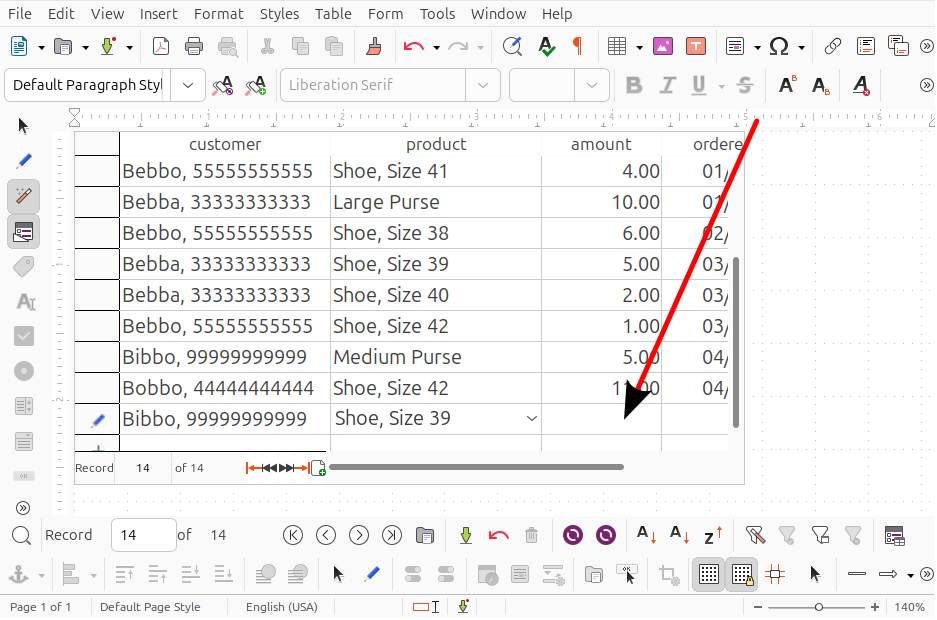
\includegraphics[width=0.49\linewidth]{\currentDir/factoryLibreOfficeBaseForms33formUseProductDone}}}%
%
\floatSep%
%
\subfloat[][%
We enter the number~7 as amount. %
We move on to the \sqlil{ordered} date field.%
\label{fig:factoryLibreOfficeBaseForms34formUseAmount}%
]{\tightbox{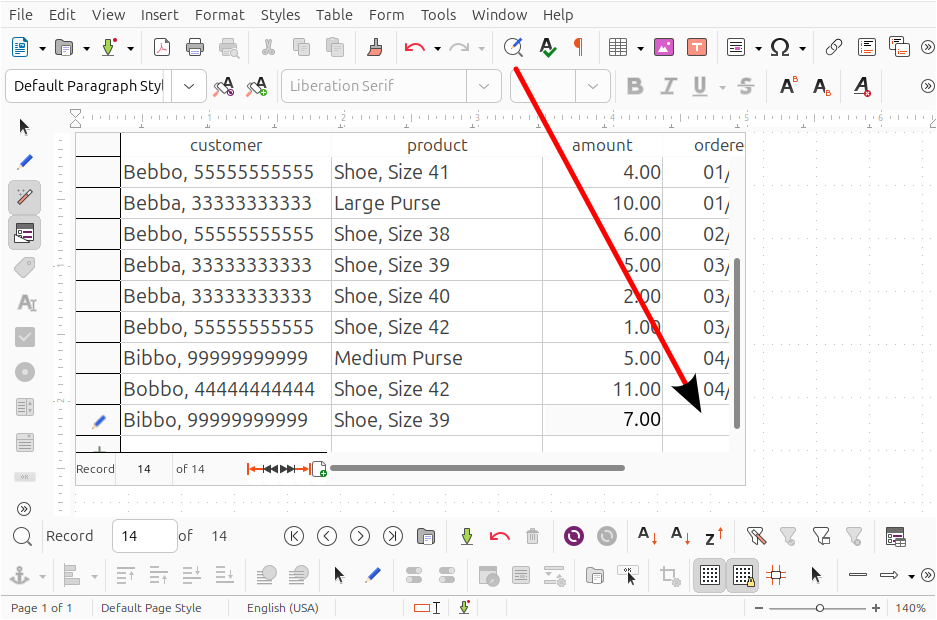
\includegraphics[width=0.49\linewidth]{\currentDir/factoryLibreOfficeBaseForms34formUseAmount}}}%
%
\floatRowSep%
%
\subfloat[][%
As order date, we type \sqlil{05/07/25}, corresponding to May~7th, 2025. %
We press~\keys{\tab}. %
The cursor jumps to a new row as our record is inserted into the \sqlil{demand} table.%
\label{fig:factoryLibreOfficeBaseForms35formUseDate}%
]{\tightbox{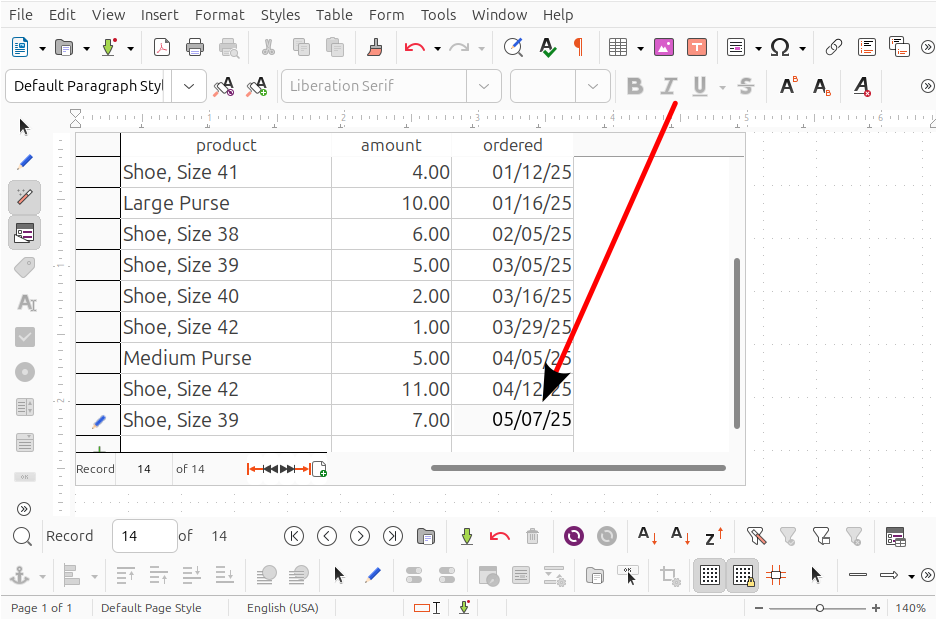
\includegraphics[width=0.49\linewidth]{\currentDir/factoryLibreOfficeBaseForms35formUseDate}}}%
%
\floatSep%
%
\subfloat[][%
We are unhappy with the way amounts and dates are displayed. %
We want to edit the form and thus click on the pencil symbol~\libreOfficeBaseDesignMode\ in the bottom bar.%
\label{fig:factoryLibreOfficeBaseForms36formUseDone}%
]{\tightbox{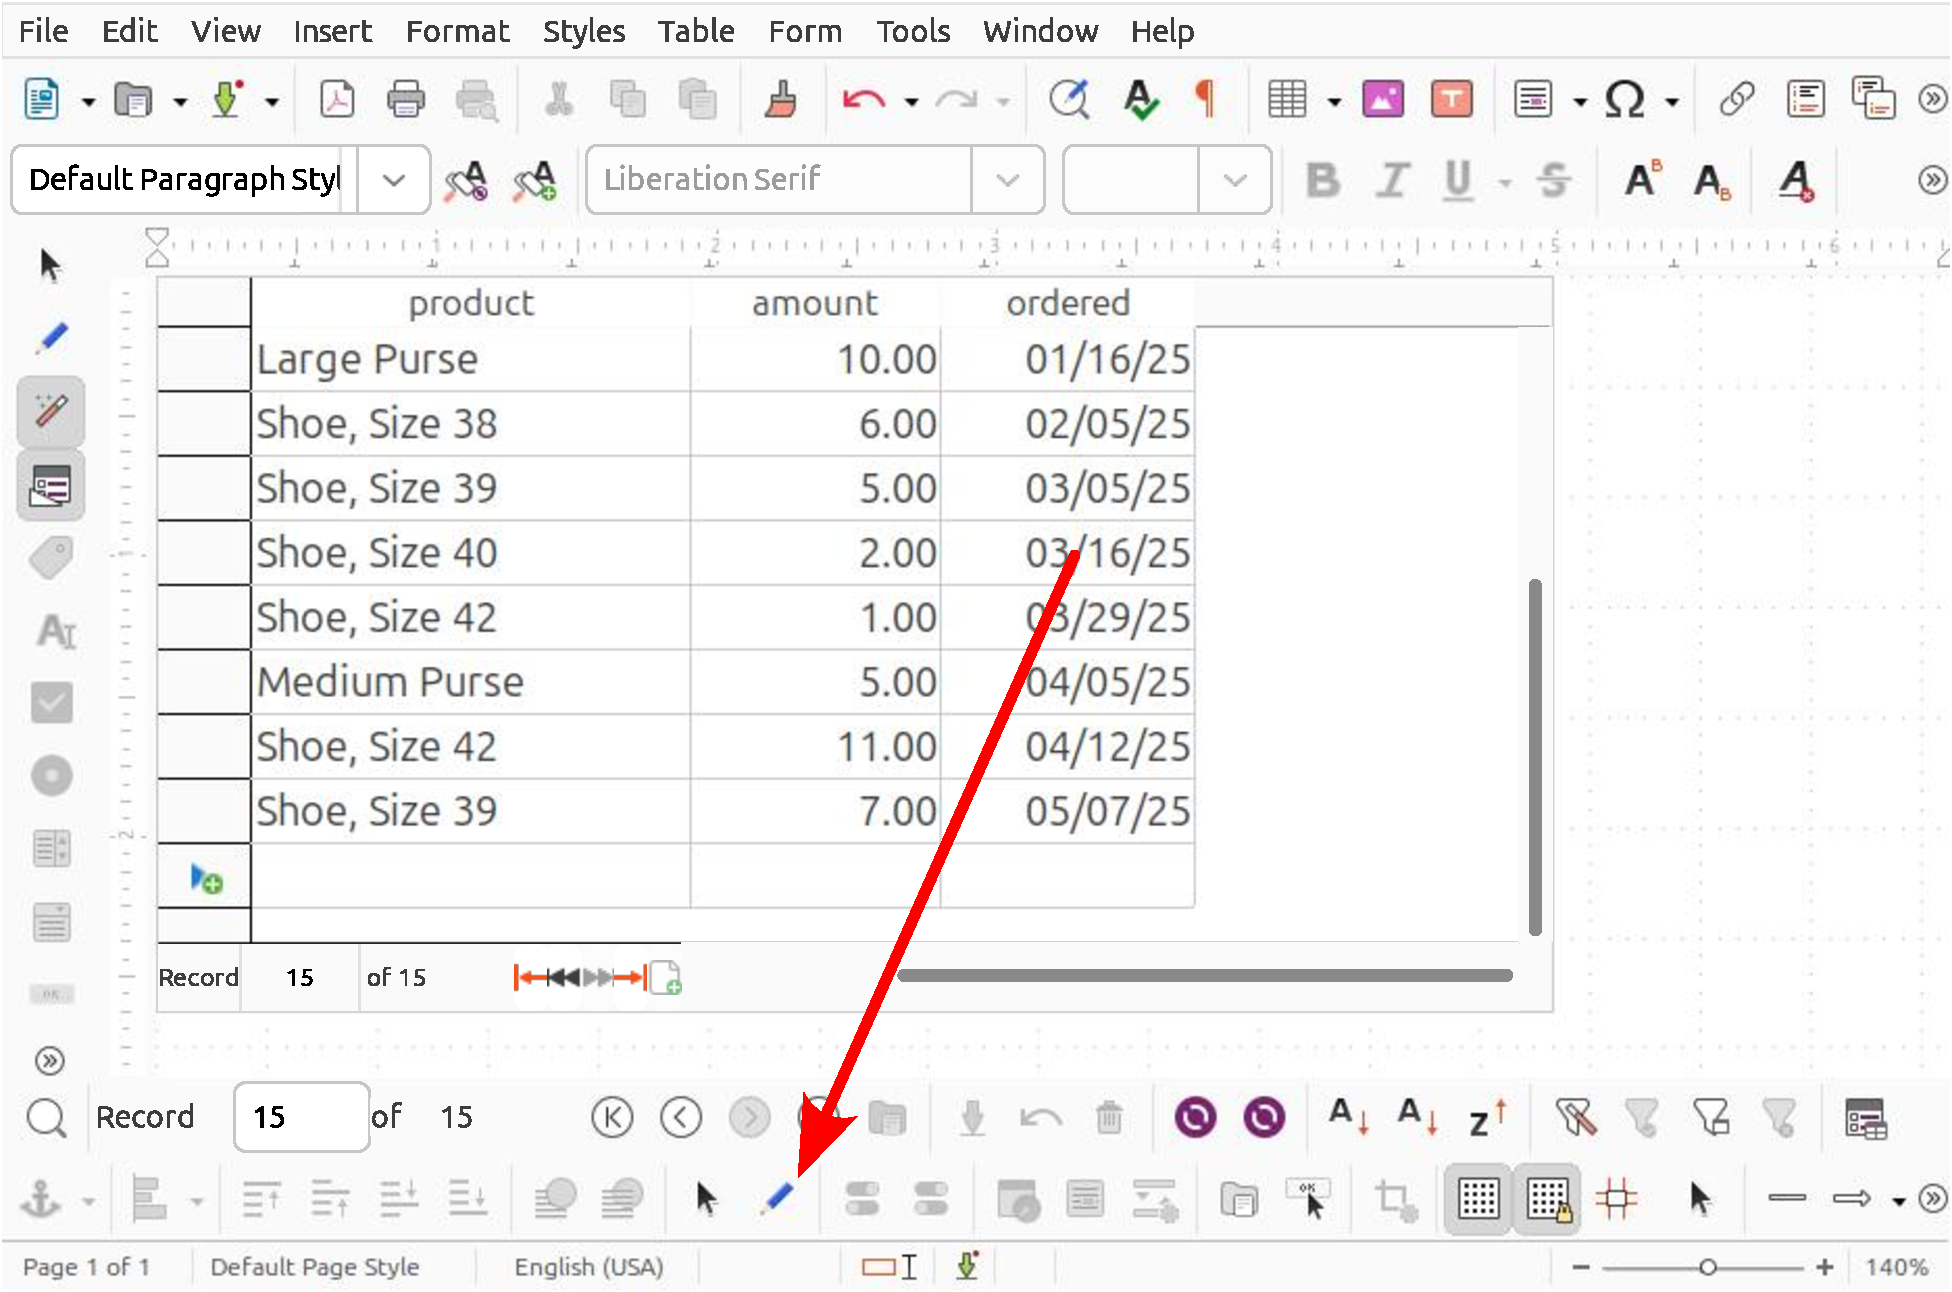
\includegraphics[width=0.49\linewidth]{\currentDir/factoryLibreOfficeBaseForms36formUseDone}}}%
%
%
\caption{Creating a form for entering demand orders into our \db\ in \libreofficeBase~(Continued).}%
\label{fig:factoryLibreOfficeBaseFormsF}%
%
\end{figure}%
%
\begin{figure}%
\ContinuedFloat%
\centering%
%
\subfloat[][%edit
The design view of the form opens again. %
We right-click on the \sqlil{amount} column.%
\label{fig:factoryLibreOfficeBaseForms37formFurtherEdit}%
]{\tightbox{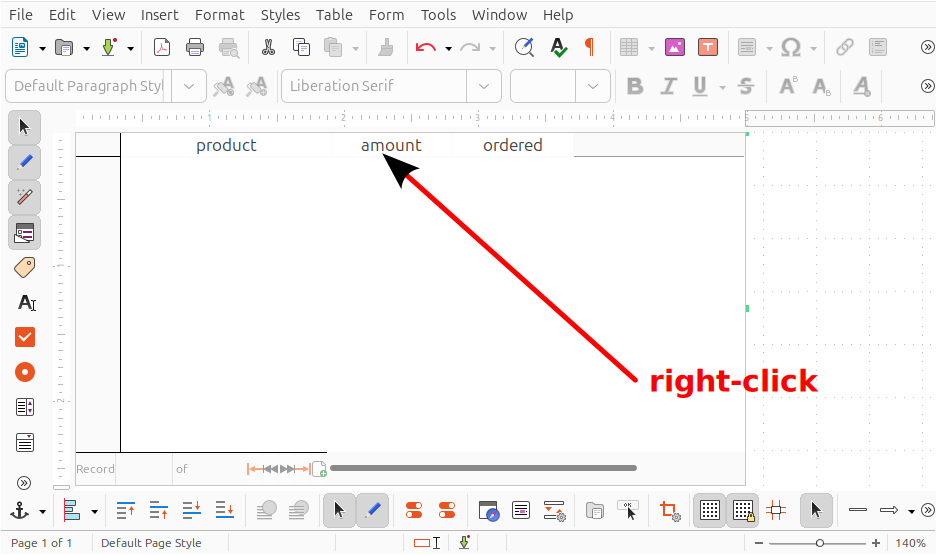
\includegraphics[width=0.49\linewidth]{\currentDir/factoryLibreOfficeBaseForms37formFurtherEdit}}}%
%
\floatSep%
%
\subfloat[][%
We click \menu{Column\dots} in the drop-down menu that opens.%
\label{fig:factoryLibreOfficeBaseForms38amountEdit}%
]{\tightbox{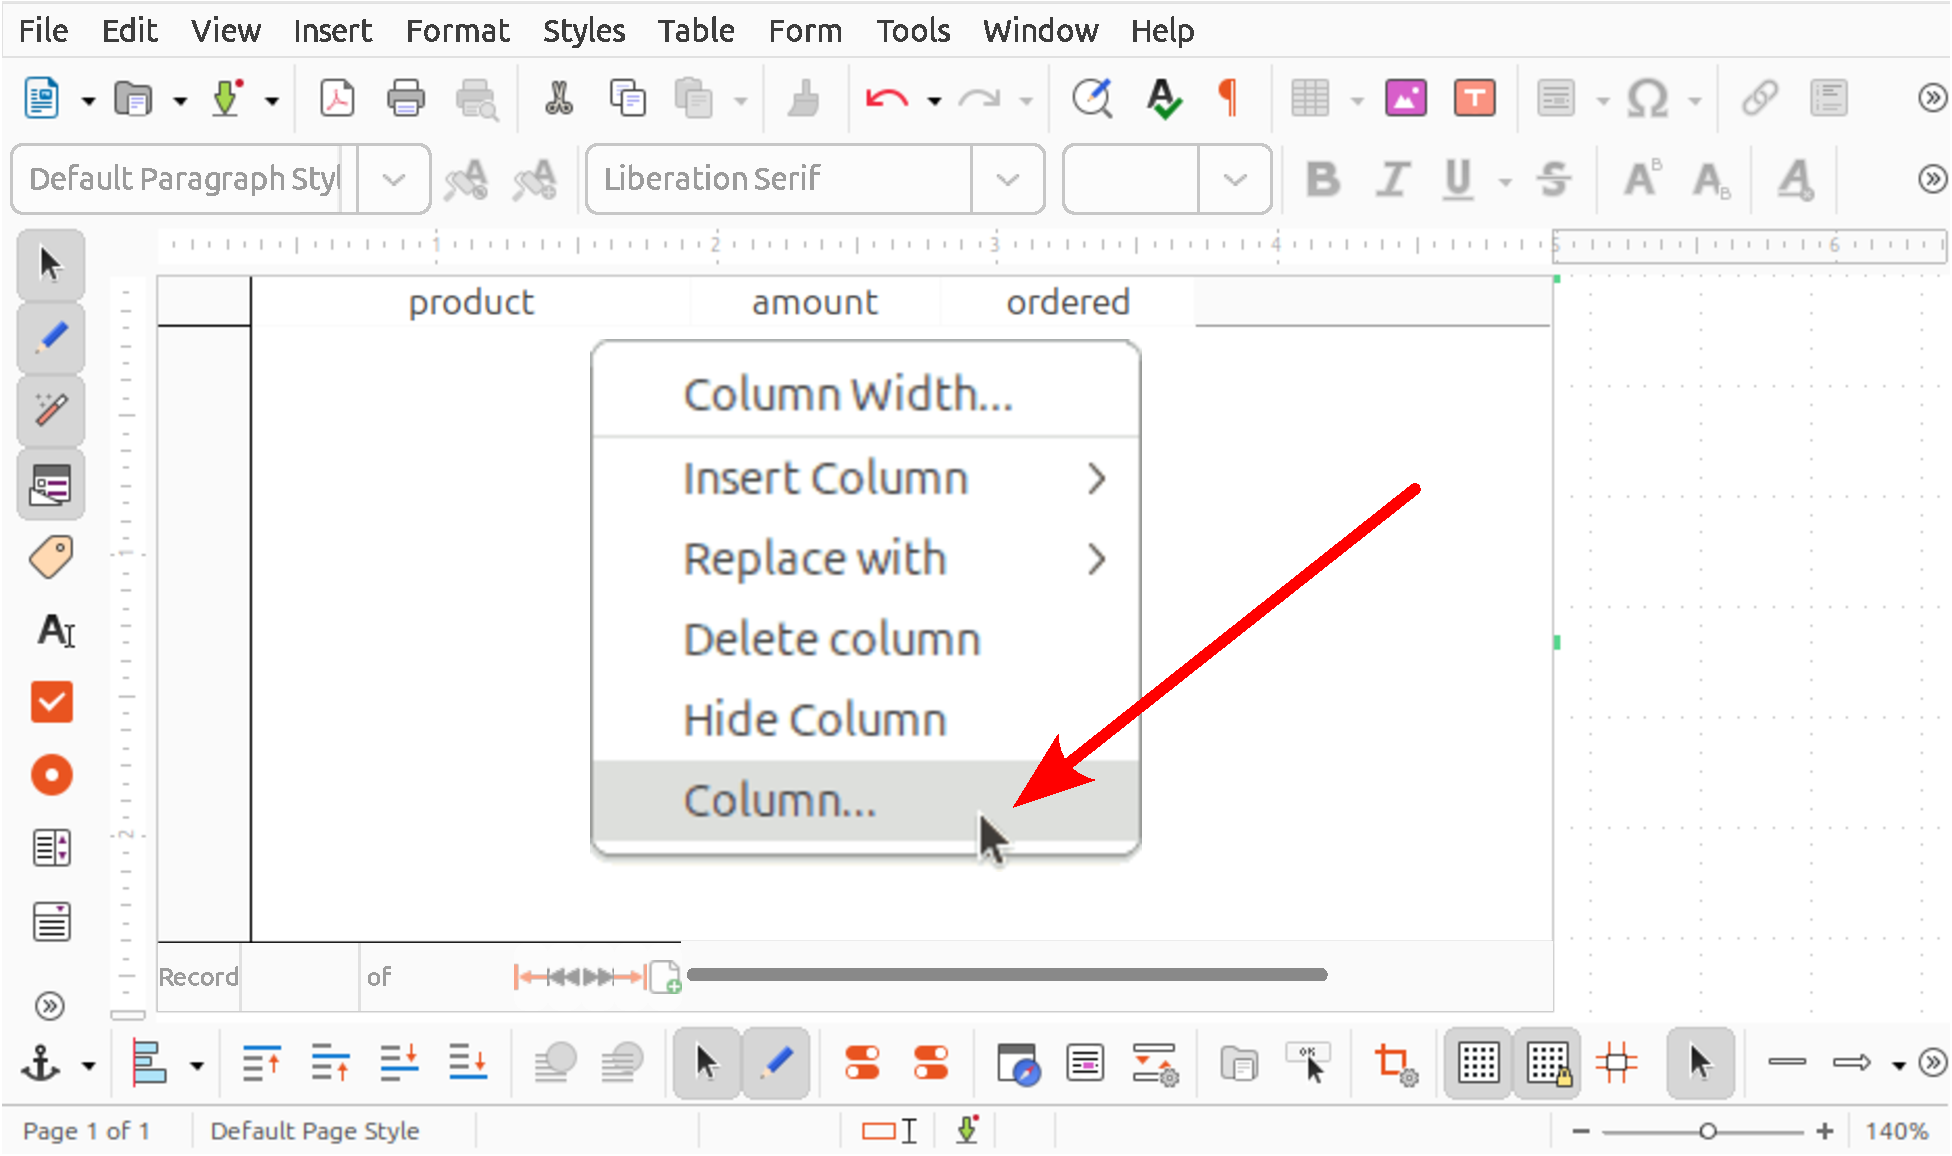
\includegraphics[width=0.49\linewidth]{\currentDir/factoryLibreOfficeBaseForms38amountEdit}}}%
%
\floatRowSep%
%
\subfloat[][%
In the \menu{General} tab, we want to change the minimal value, the decimal accuracy, and the thousand separator setting.%
\label{fig:factoryLibreOfficeBaseForms39amountSettings}%
]{\tightbox{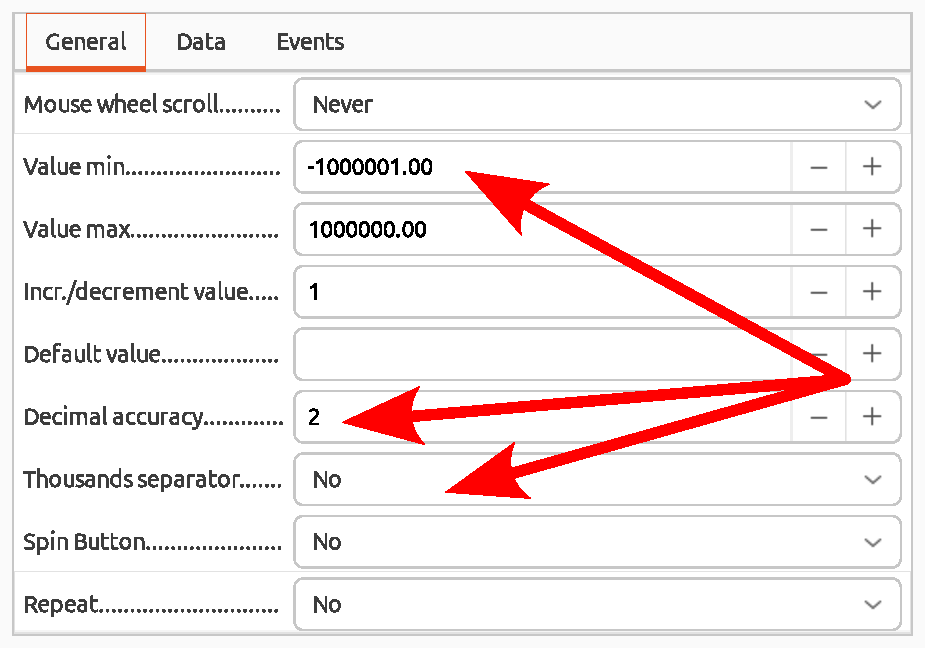
\includegraphics[width=0.49\linewidth]{\currentDir/factoryLibreOfficeBaseForms39amountSettings}}}%
%
\floatSep%
%
\subfloat[][%
The minimum gets set to~0. %
We do not allow fractions, so the decimal accuracy becomes~0. %
For the case that someone orders thousands of shoes, we would display a thousand separator. %
We close this dialog.%
\label{fig:factoryLibreOfficeBaseForms40amountFixed}%
]{\tightbox{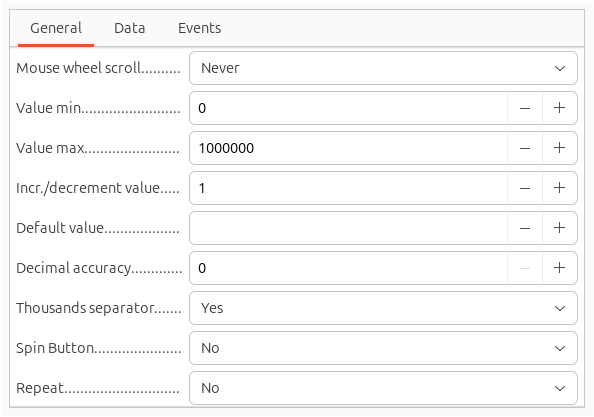
\includegraphics[width=0.49\linewidth]{\currentDir/factoryLibreOfficeBaseForms40amountFixed}}}%
%
\floatRowSep%
%
\subfloat[][%
We now right-click on the \sqlil{ordered} column.%
\label{fig:factoryLibreOfficeBaseForms41editOrdered}%
]{\tightbox{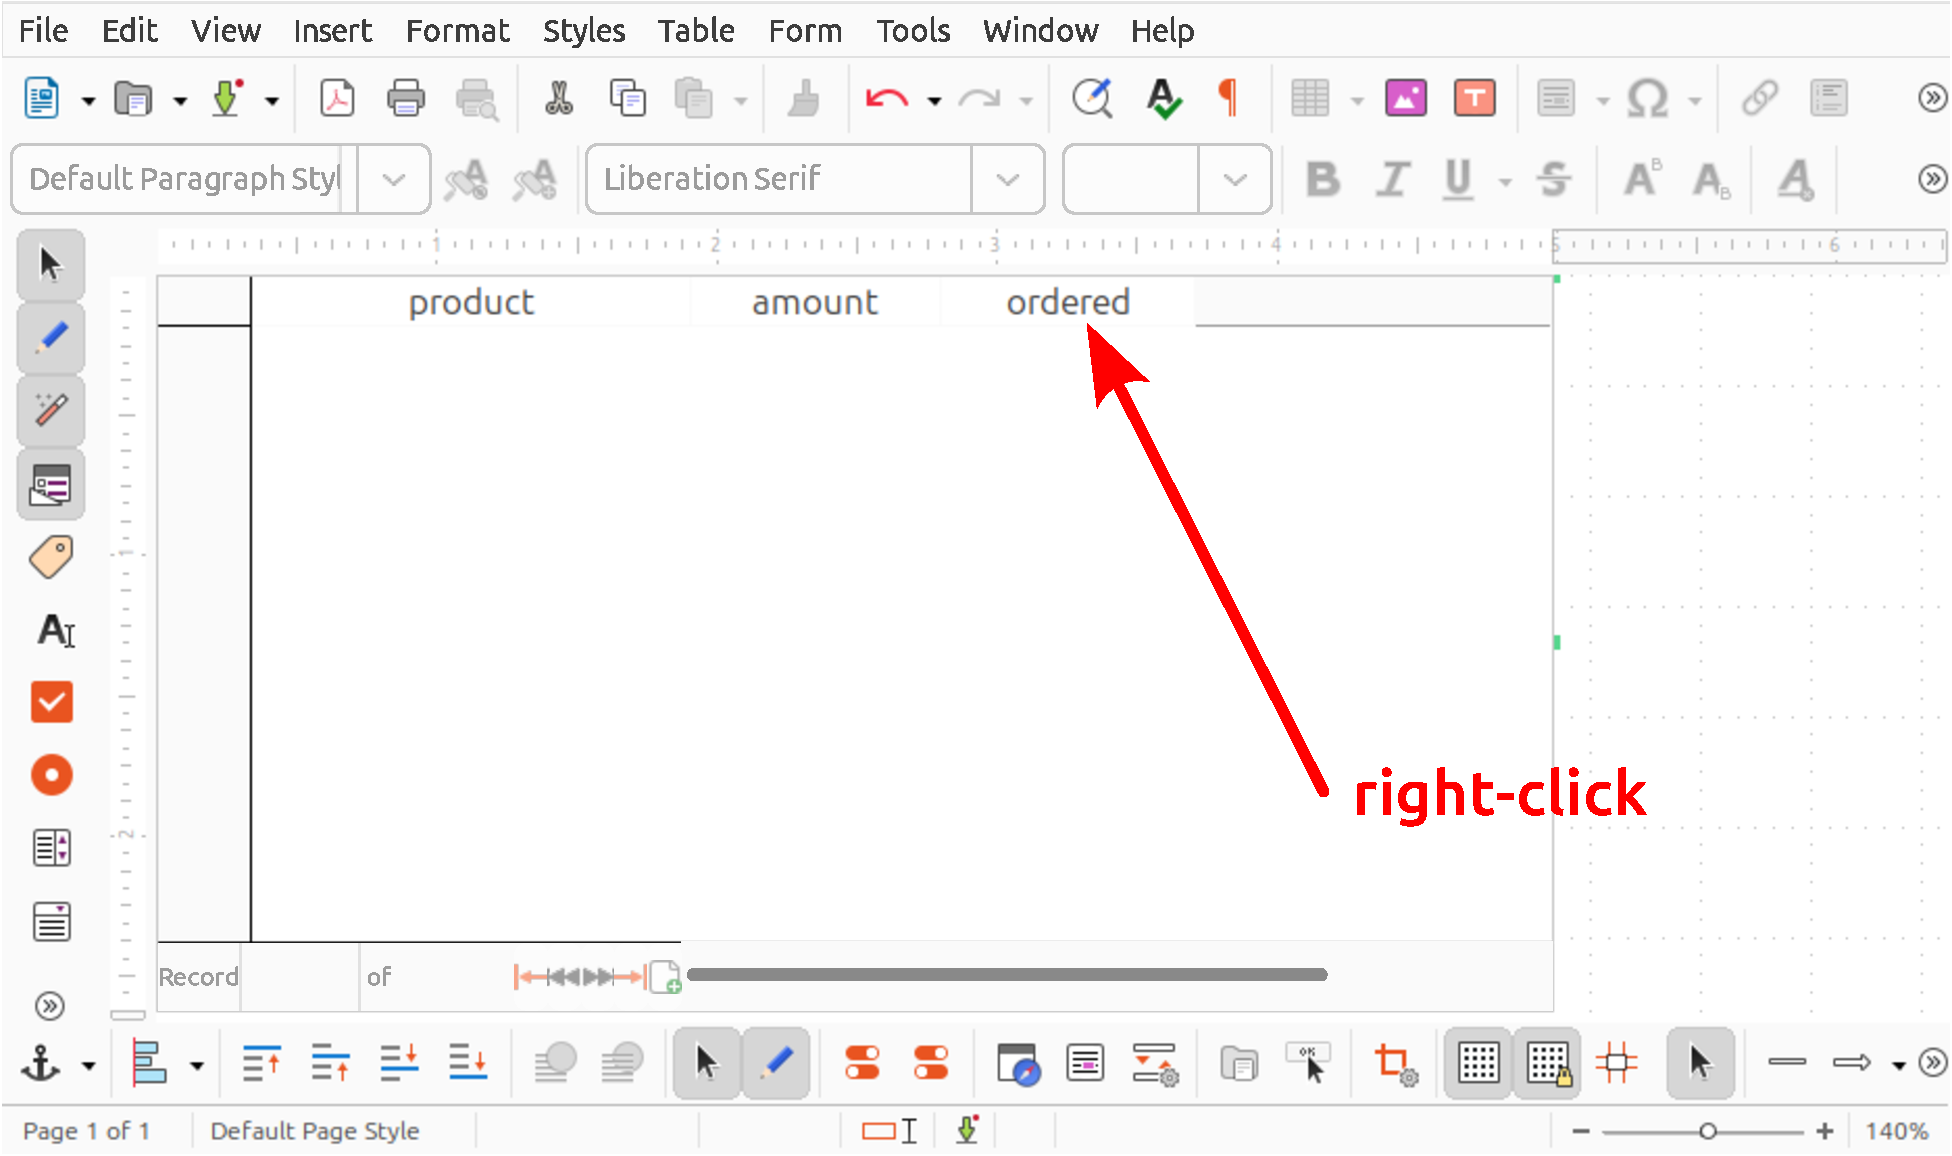
\includegraphics[width=0.49\linewidth]{\currentDir/factoryLibreOfficeBaseForms41editOrdered}}}%
%
\floatSep%%
%
\subfloat[][%
In the drop-down menu that opens, we click \menu{Column\dots}.%
\label{fig:factoryLibreOfficeBaseForms42orderedEdit}%
]{\tightbox{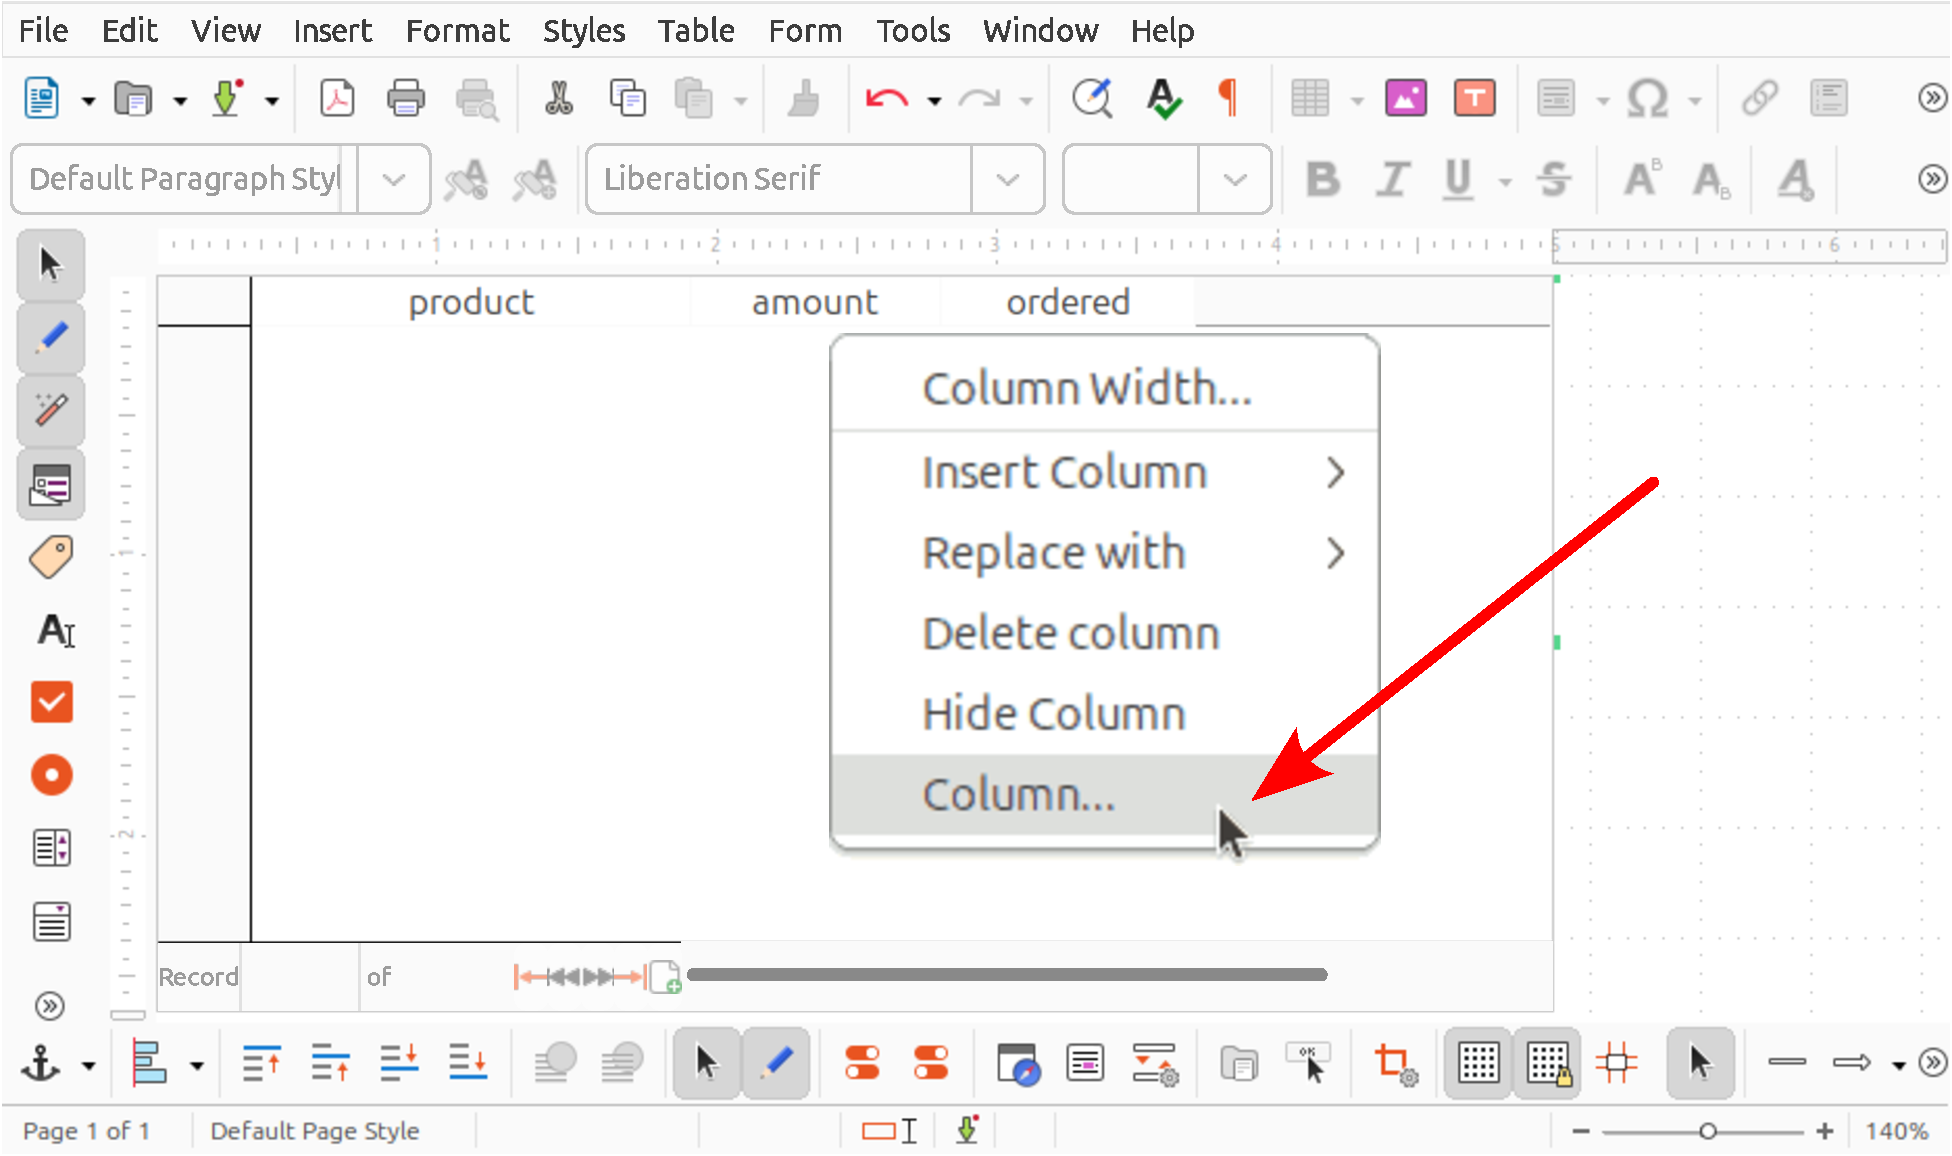
\includegraphics[width=0.49\linewidth]{\currentDir/factoryLibreOfficeBaseForms42orderedEdit}}}%
%
%
\caption{Creating a form for entering demand orders into our \db\ in \libreofficeBase~(Continued).}%
\label{fig:factoryLibreOfficeBaseFormsG}%
%
\end{figure}%
%
\begin{figure}%
\ContinuedFloat%
\centering%
%
\subfloat[][%
In the \menu{General} pane, we want to change the \emph{Date format} and not use this awful short US~format.%
\label{fig:factoryLibreOfficeBaseForms43orderedSettings}%
]{\tightbox{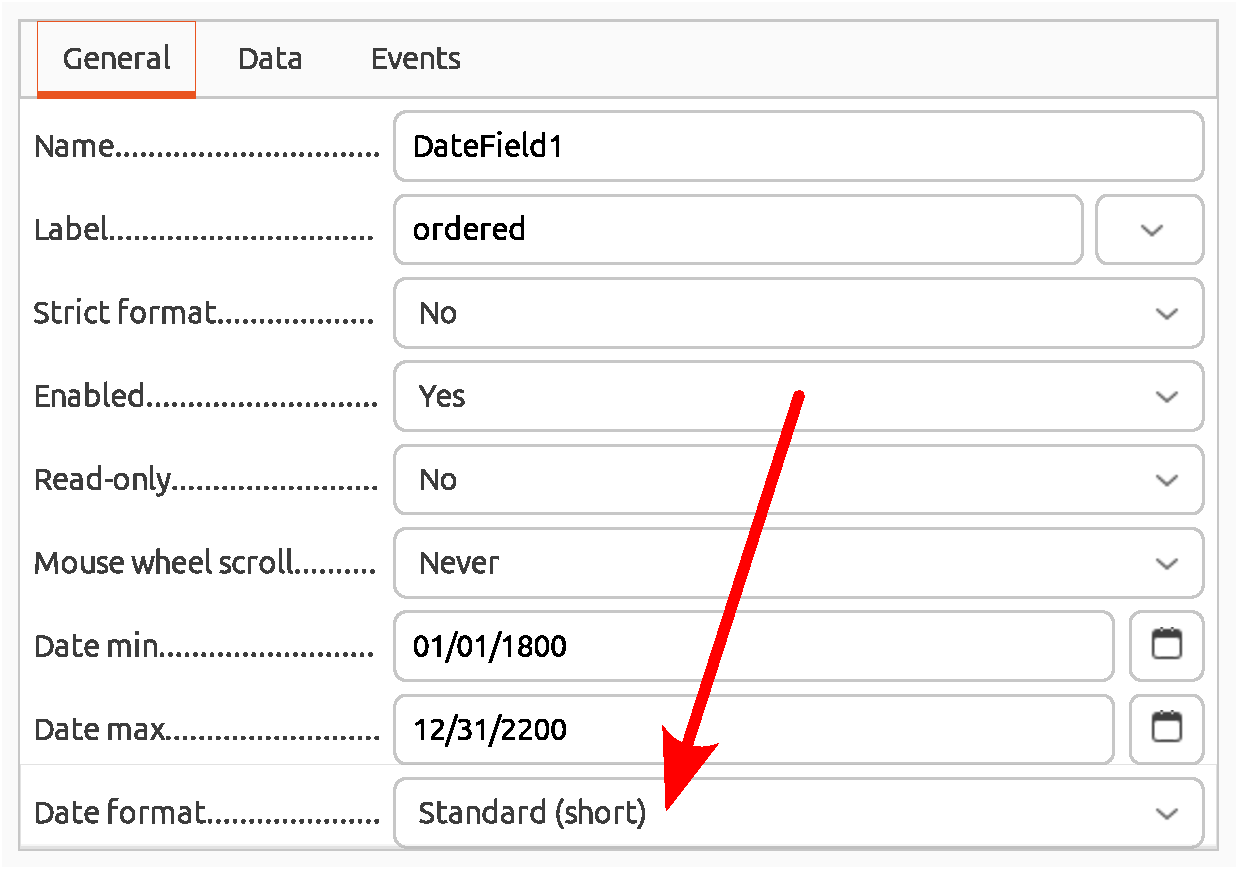
\includegraphics[width=0.49\linewidth]{\currentDir/factoryLibreOfficeBaseForms43orderedSettings}}}%
%
\floatSep%
%
\subfloat[][%
We set the date format to \inQuotes{YYYY-MM-DD}, which is the same format used in our \sql\ queries. %
We close the dialog.%
\label{fig:factoryLibreOfficeBaseForms44orderedFixed}%
]{\tightbox{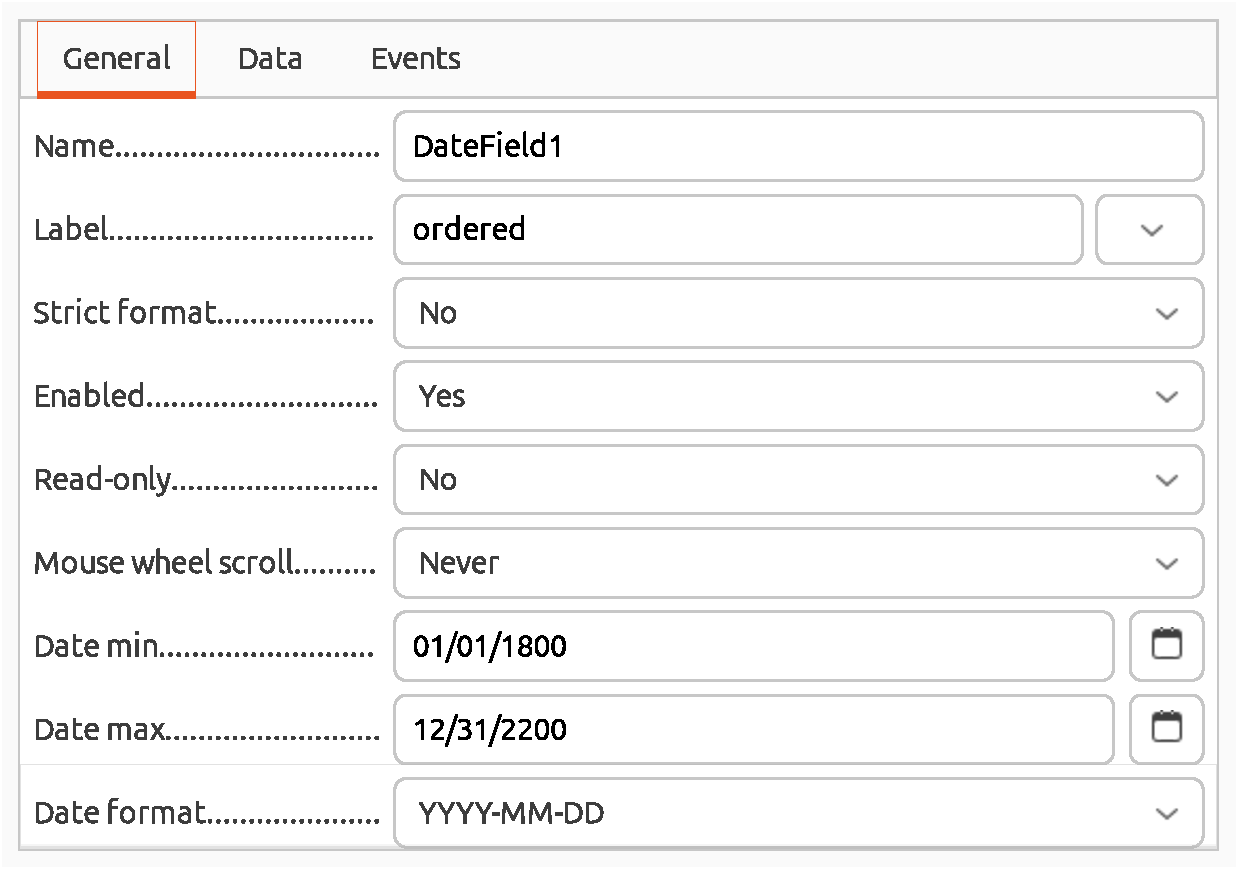
\includegraphics[width=0.49\linewidth]{\currentDir/factoryLibreOfficeBaseForms44orderedFixed}}}%
%
\floatRowSep%
%
\subfloat[][%
We also want to make the form a bit wider. %
We click on the green handle in the middle of the right side of the table area and drag it outwards. %
After releasing it, we again click on the pencil symbol~\libreOfficeBaseDesignMode\ to leave the design view.%
\label{fig:factoryLibreOfficeBaseForms45wider}%
]{\tightbox{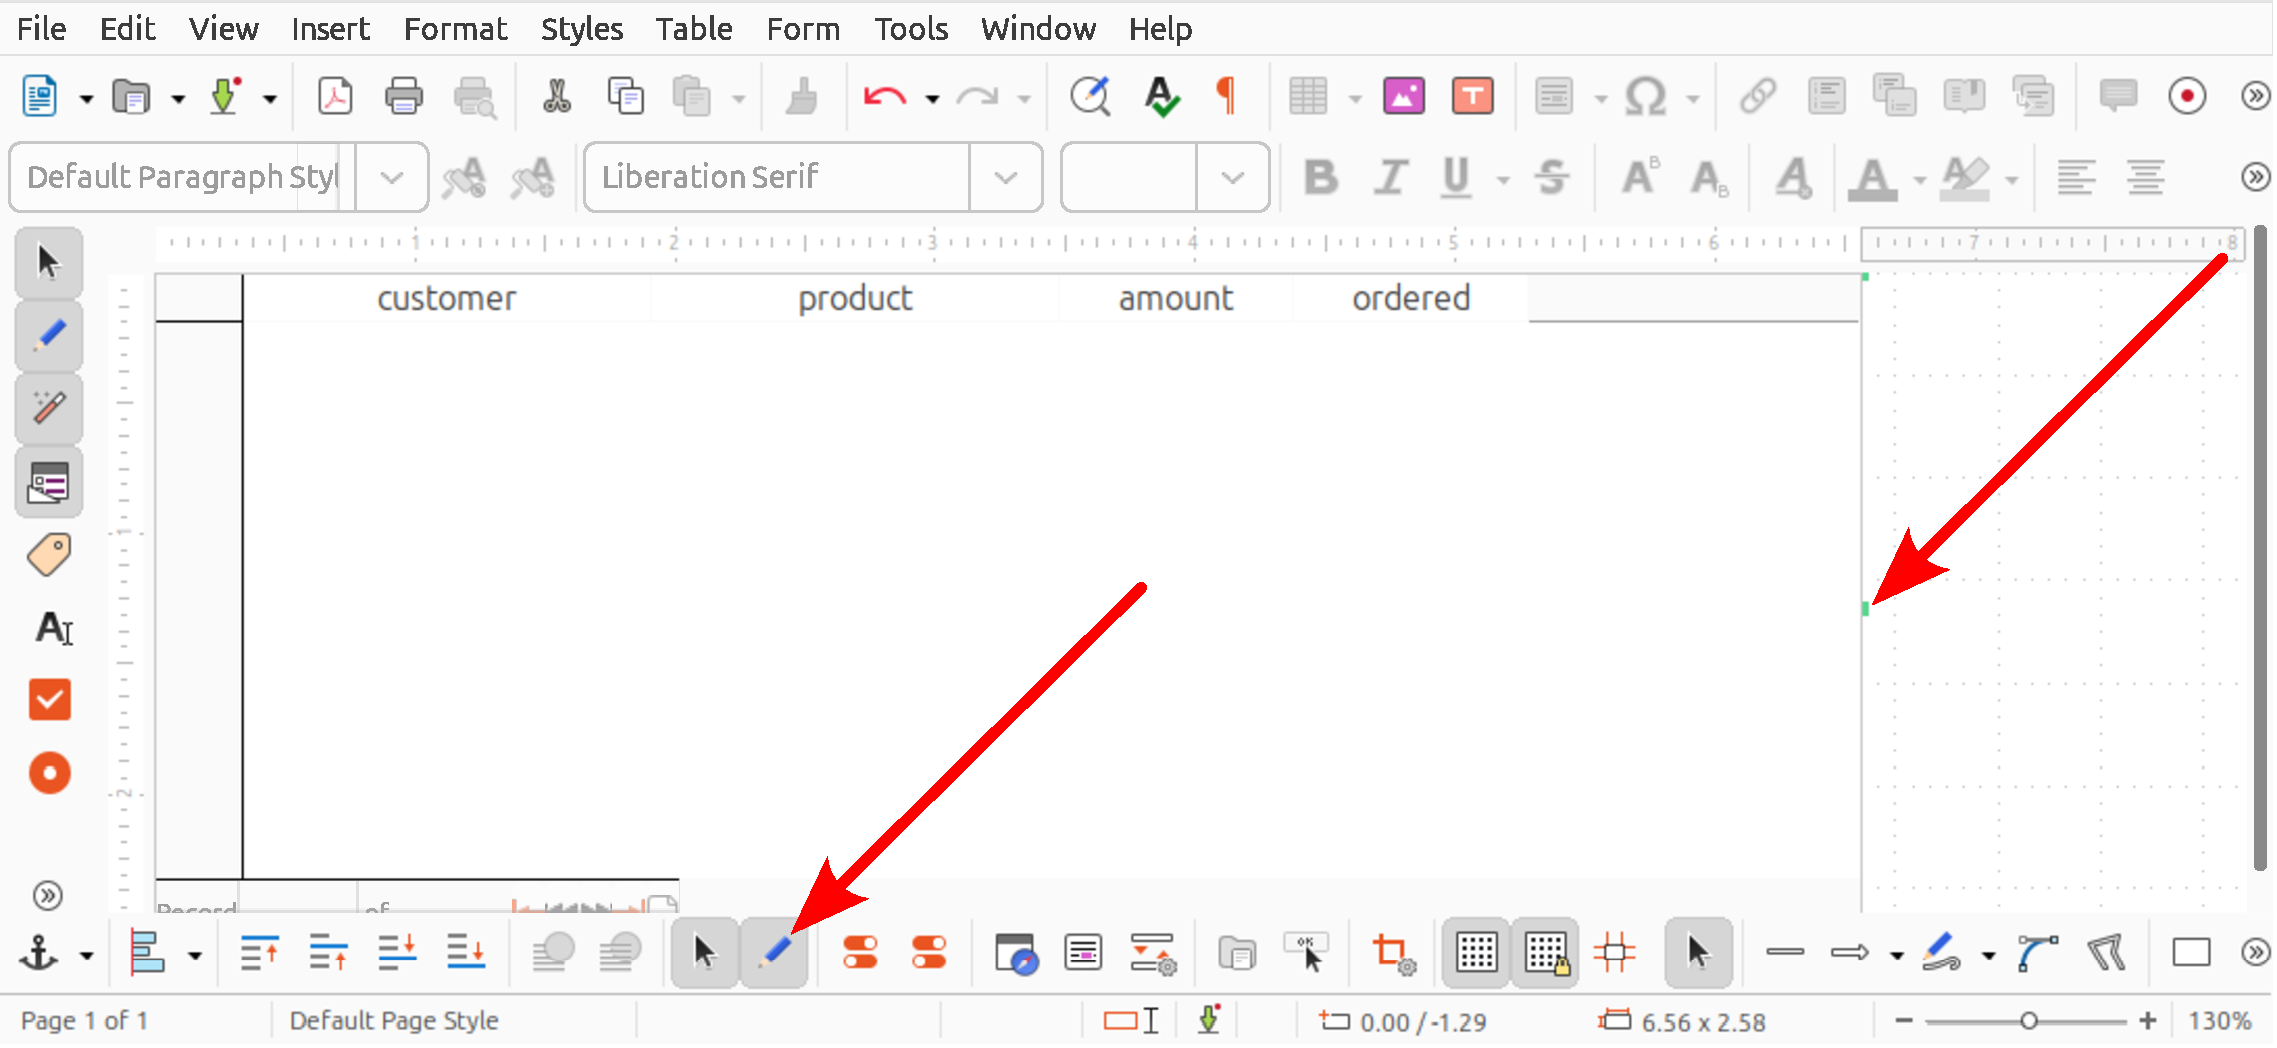
\includegraphics[width=0.49\linewidth]{\currentDir/factoryLibreOfficeBaseForms45wider}}}%
%
\floatSep%
%
\subfloat[][%
The form is again displayed \inQuotes{in action.} %
It looks very nice now. %
We are done with our work.%
\label{fig:factoryLibreOfficeBaseForms46editDone}%
]{\tightbox{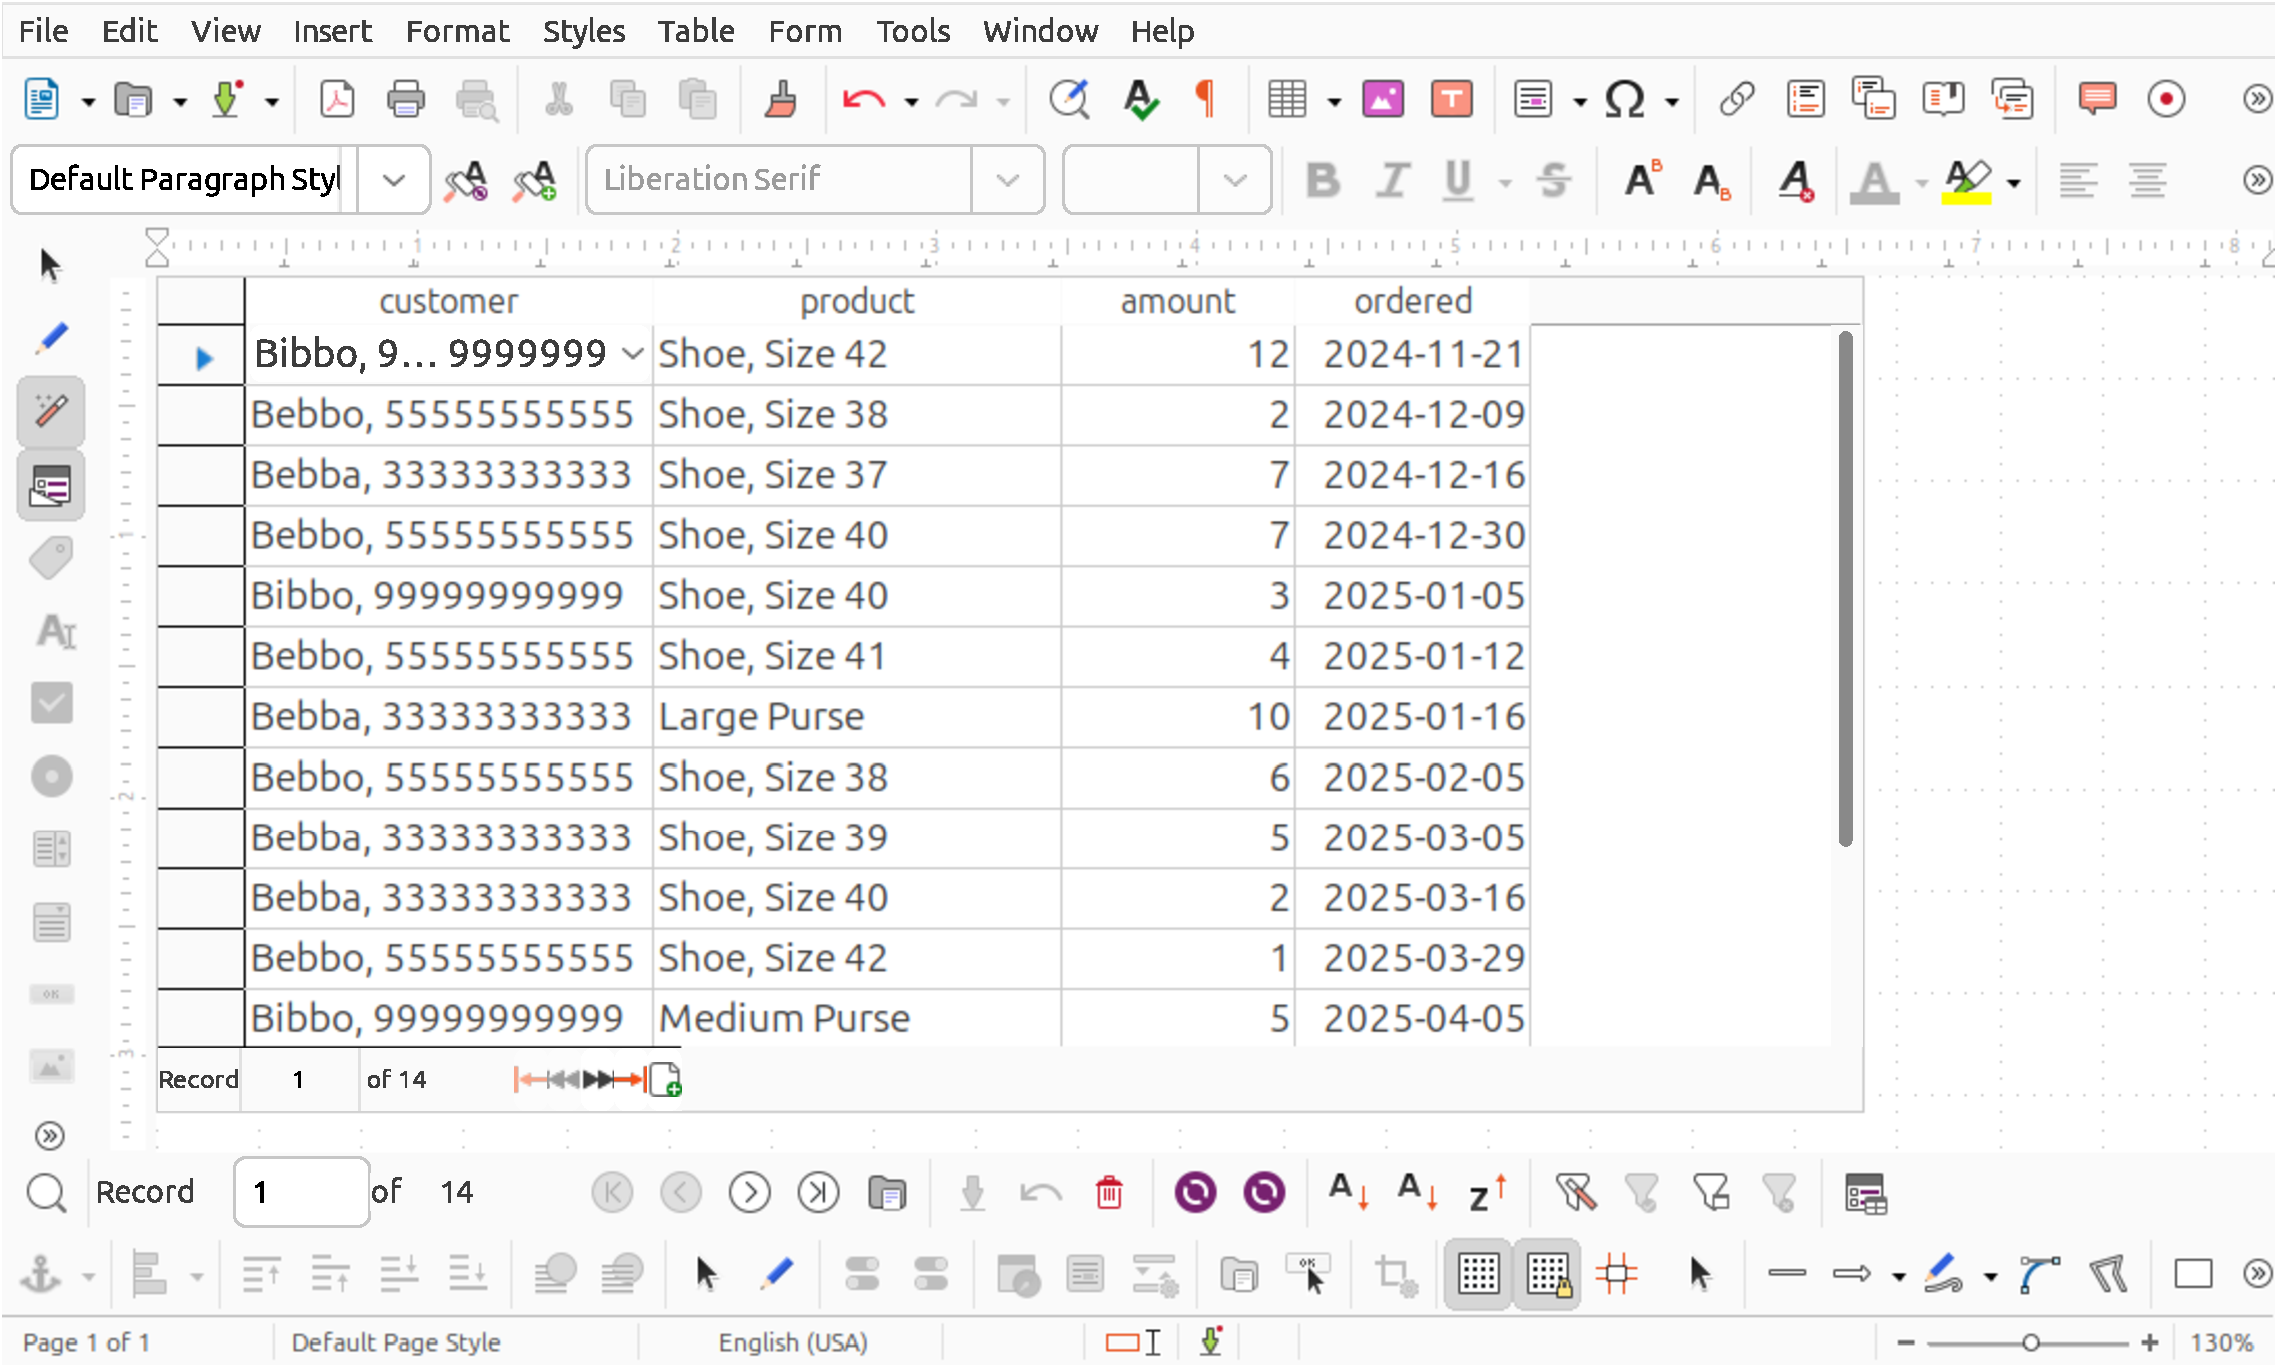
\includegraphics[width=0.49\linewidth]{\currentDir/factoryLibreOfficeBaseForms46editDone}}}%
%
\floatRowSep%
%
\subfloat[][%
We close the form. %
We get asked whether want to save it. %
We of course click on \menu{Save}.%
\label{fig:factoryLibreOfficeBaseForms47closingSave}%
]{\tightbox{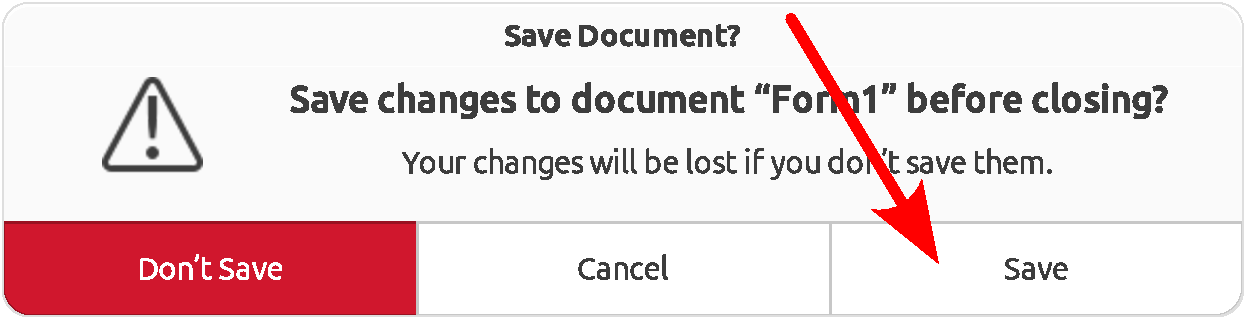
\includegraphics[width=0.49\linewidth]{\currentDir/factoryLibreOfficeBaseForms47closingSave}}}%
%
\floatSep%
%
\subfloat[][%
We choose the name \sqlil{demand} for our form and type this into the \emph{File name:}~box. %
We click \menu{Save}.%
\label{fig:factoryLibreOfficeBaseForms48saveAsDemand}%
]{\tightbox{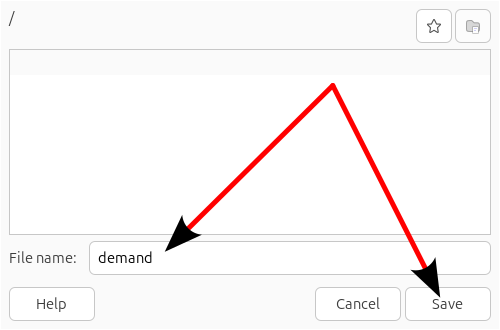
\includegraphics[width=0.49\linewidth]{\currentDir/factoryLibreOfficeBaseForms48saveAsDemand}}}%
%
%
\caption{Creating a form for entering demand orders into our \db\ in \libreofficeBase~(Continued).}%
\label{fig:factoryLibreOfficeBaseFormsH}%
%
\end{figure}%
%
\begin{figure}%
\ContinuedFloat%
\centering%
%
\subfloat[][%
We are back in the main window of \libreofficeBase. %
Let's click again on our new \sqlil{demand} form to see whether it is still there and whether it still works.%
\label{fig:factoryLibreOfficeBaseForms49forms}%
]{\tightbox{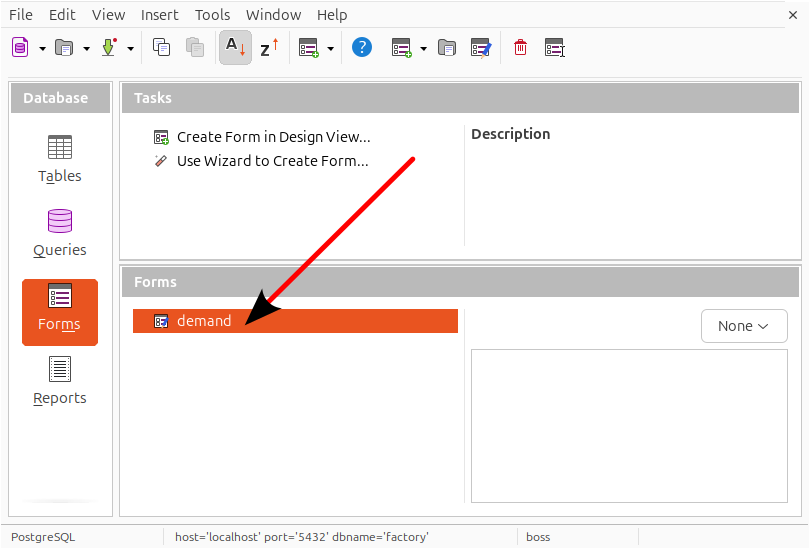
\includegraphics[width=0.49\linewidth]{\currentDir/factoryLibreOfficeBaseForms49forms}}}%
%
\floatSep%
%
\subfloat[][%
The form opens in all of its beauty.%
\label{fig:factoryLibreOfficeBaseForms50reopened}%
]{\tightbox{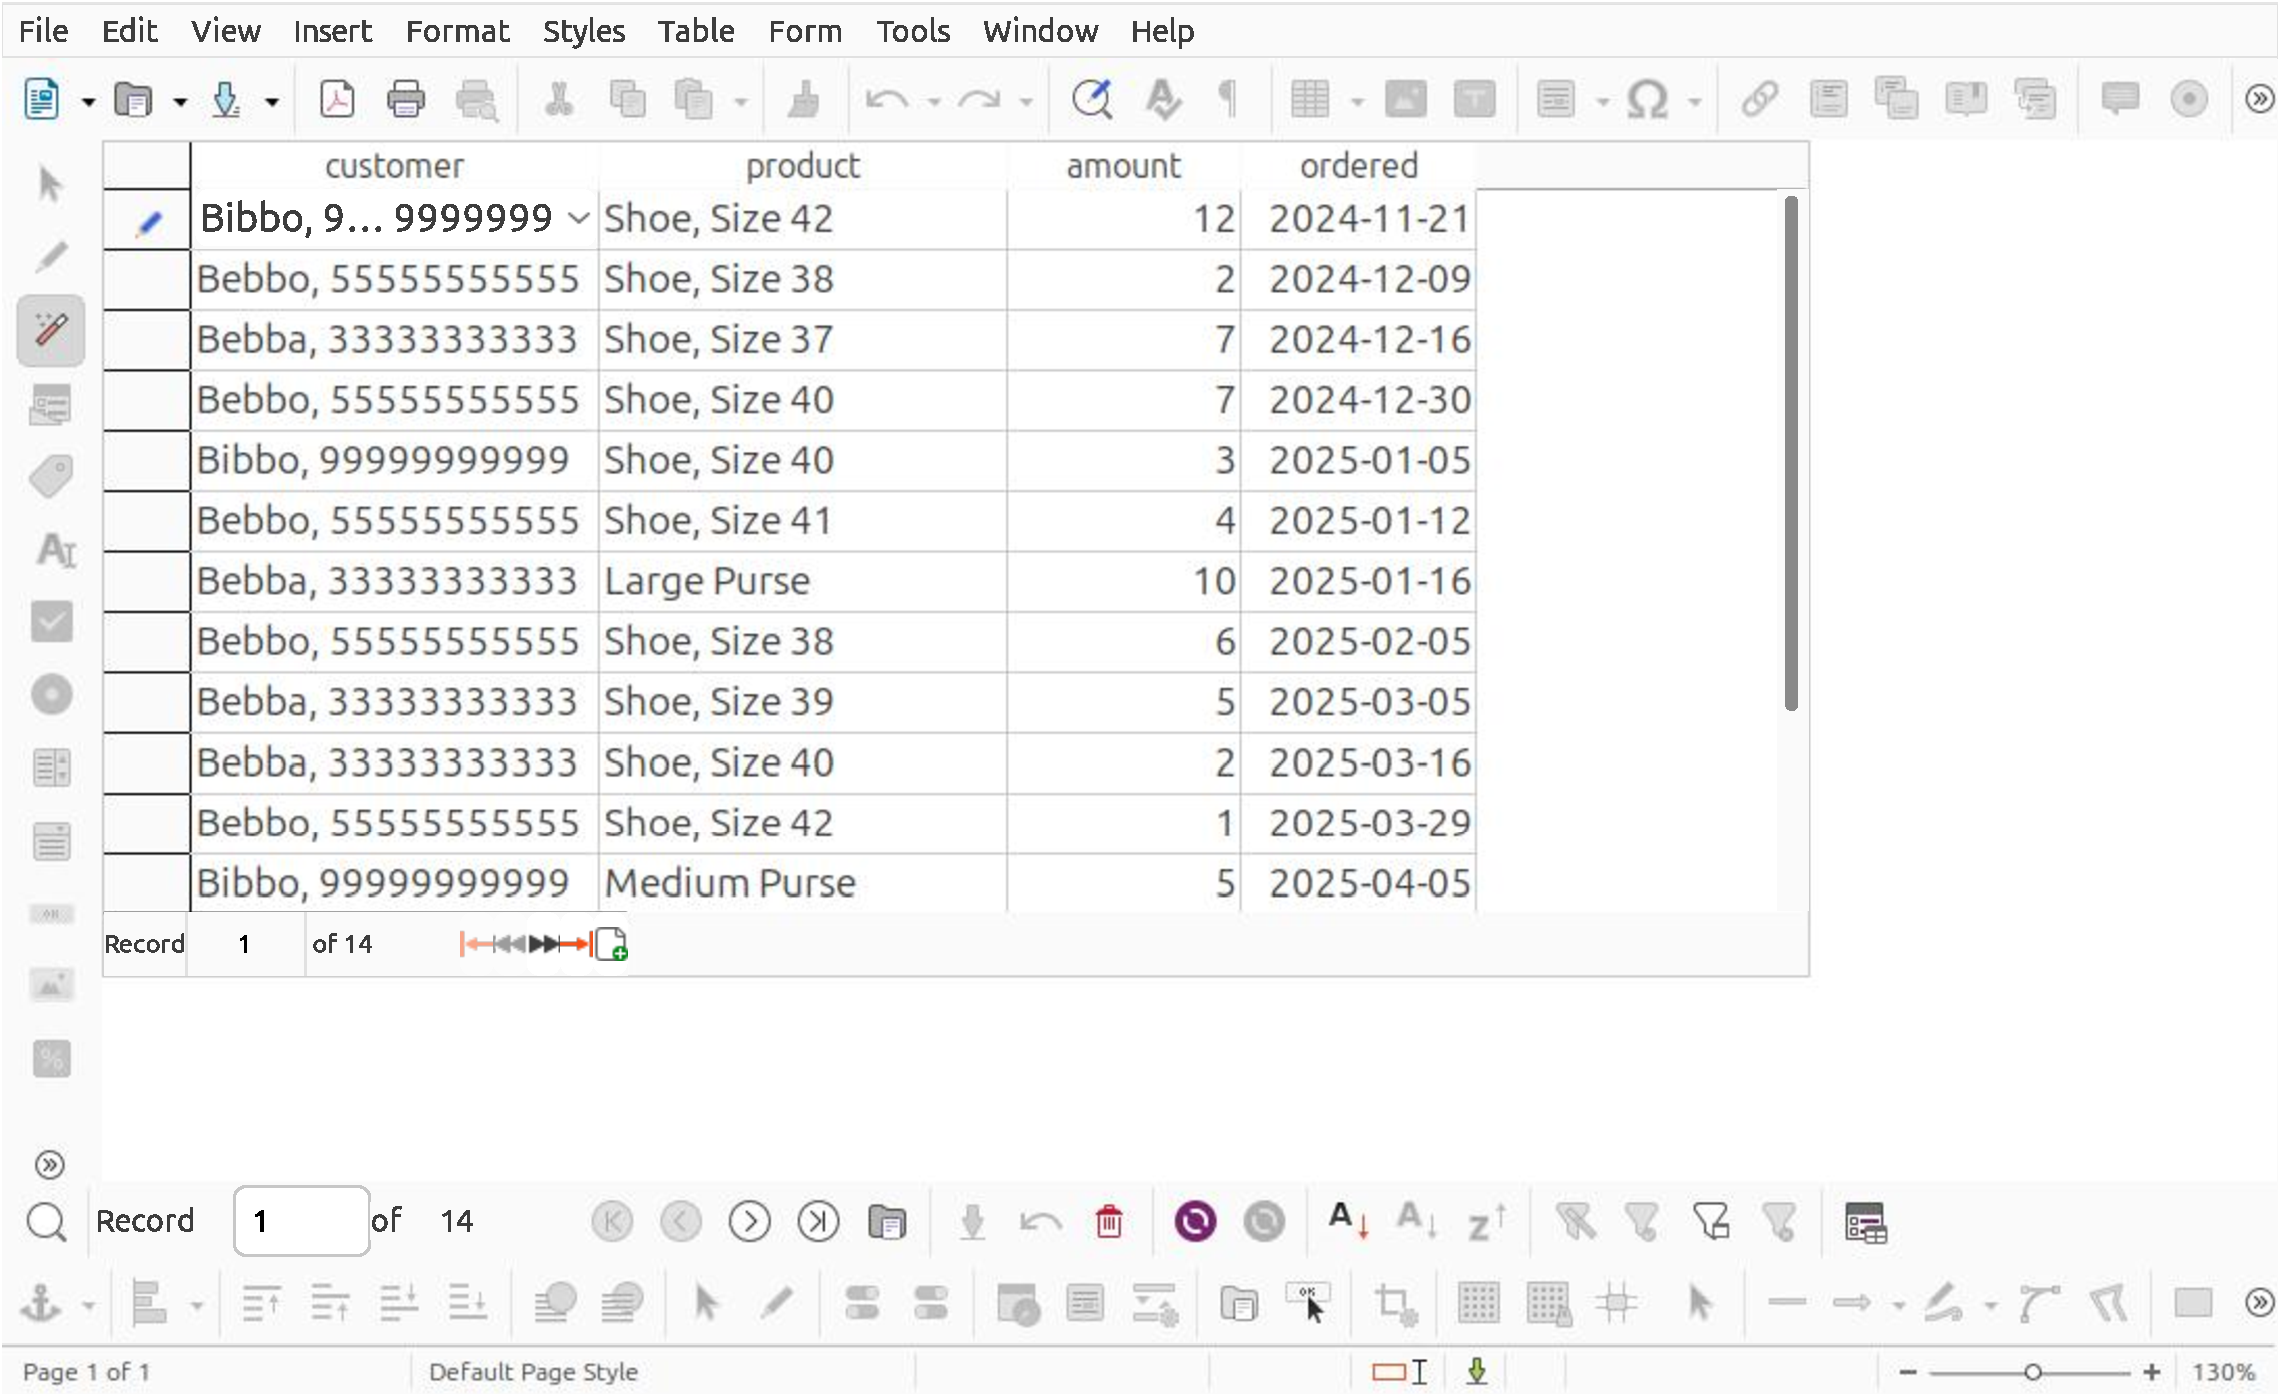
\includegraphics[width=0.49\linewidth]{\currentDir/factoryLibreOfficeBaseForms50reopened}}}%
%
%
\caption{Creating a form for entering demand orders into our \db\ in \libreofficeBase~(Continued).}%
\label{fig:factoryLibreOfficeBaseFormsI}%
%
\end{figure}%
%
%
At some point in this example, we realized that entering data into a \db\ via a \sql\ \client\ like \psql\ is maybe not a very convenient way.
In \cref{sec:factory:tableAndView}, we found that we can also enter data into tables in a much more convenient way by typing it in a table-based \pgls{GUI}.
This is a big step forward, because it does not require any understanding of \sql.
We, as the \pglspl{dba}, can create and manage a \db\ using \sql.
Then we can connect a frontend like \libreofficeBase\ to it and give this as \client\ to a secretary.
They can then enter the data in a way that is more natural to them.
Our \db\ will stay consistent and the data integrity is preserved by its constraints.
This is much better than an \microsoftExcel\ sheet or that alike.
Multiple people can work with \db\ concurrently using the \pglspl{client} on multiple computers.
Different types of related data can be entered simulataneously.
Also, it is much harder to create invalid data.

However, entering records with foreign keys is still a total buzzkill.
This comes to light when dealing with table \sqlil{demand}.
The user needs to keep the tables \sqlil{product} and \sqlil{customer} open, too.
They need to look up customer~ids and product~ids and use them manually.
And there is no protection against entering the id of the wrong customer or product.
While we can pull the data together nicely in the view \sqlil{sale} once it is entered{\dots}
{\dots}we do not have a way to enter it comfortably.
Not yet.

Because now we learn an easy way to build an input method for datasets with foreign keys.
This method is called \emph{forms}.
Both \microsoftAccess\ and \libreofficeBase\ allow us to develop so-called forms.
Forms are entry masks that can be designed in different ways.
We can place different controls onto forms.
The controls may take their data from different tables in the \db.
This is what we are after.
So we will now design a form for entering customer demands into our \db\ from \libreofficeBase.

We therefore first open our dokument \textil{factory.odb} using \libreofficeBase.
To connect with the \db, we will have to enter the password \textil{superboss123}.
In the \menu{Database} pane on the right-hand side of the \libreofficeBase\ window, we select \menu{For\underline{m}s}.
Then, under \menu{Tasks}, we  click on \inQuotes{Create Form in Design View\dots} in \cref{fig:factoryLibreOfficeBaseForms01createInDesignView}.
Then, in \cref{fig:factoryLibreOfficeBaseForms02designView}, a new and empty form opens in the design view.
Now there are several different possible structures in which we can create a form.
Forms can look like the classical dialogs that we used so far in \libreoffice.
Or they can look more like the tables-based view that we used to enter demand orders manually in \cref{sec:factory:tableAndView}.
We want to design a form following this structure, but we want to make it more easy to use, of course.
Therefore, we will insert a table control, which can be reached by the button~\libreOfficeBaseTable.
Depending on your screen size, this button may be directly located on the control palette on the left-hand side of the screen.
Or, as is the case on my screen, may be hidden behind double-angle button~\libreOfficeBaseMore\ near the bottom of the control palette.
In \cref{fig:factoryLibreOfficeBaseForms03insertTable}, we click on that button, a small window with additional controls opens, and then we click on on the table control button~\libreOfficeBaseTable.

We now click into the empty form body and drag the mouse to span a reasonably sized area before releasing the button in \cref{fig:factoryLibreOfficeBaseForms04insertTable}.
A dialog opens in \cref{fig:factoryLibreOfficeBaseForms05selectSource}.
It asks about the data we want to use in the table control.
In other words, we now need to link our table \emph{control} to a table in our \emph{\db}.
There are lots of tables we can select from.
Most of them are storing some meta-data about the \db\ and are not for us to meddle with.
All of \inQuotes{our} tables are available under the prefix \sqlil{public}
We scroll down all the way in the view on the right side and select \sqlil{public.demand}.
Then we click \menu{Next}.

In the next dialog depicted in \cref{fig:factoryLibreOfficeBaseForms06tableElements} we can select columns to insert.
We only choose \sqlil{amount} and \sqlil{ordered}.
As said, we want to be able to enter the \sqlil{customer} and \sqlil{product} field not as numbers.
Therefore, we will not include them here.
We will design specialized controls for them later.
We click \menu{Finish}.

The table control is now inserted in draft form in \cref{fig:factoryLibreOfficeBaseForms07table}.
It has the two columns \sqlil{amount} and \sqlil{ordered} as prescribed.
Now we want to add columns for \sqlil{customer} and \sqlil{product}.
Therefore, we right-click at the left corner of the \sqlil{amount} column.

In the menu that opens, click \menu{Insert Column} and then \menu{List Box} in \cref{fig:factoryLibreOfficeBaseForms08addListColumn}.
Indeed, back to the draft of our form in \cref{fig:factoryLibreOfficeBaseForms09listColumnAdded}, we can see that a new column named \inQuotes{List Box 1} has been added.
We right-click on it.
In the menu that opens in \cref{fig:factoryLibreOfficeBaseForms10editListColumn}, we click on \menu{Column...}.
A new dialog opens up in which we can configure the new column.
As shown in \cref{fig:factoryLibreOfficeBaseForms11generalOld}, we first select the \menu{General} tab in this dialog.
We change both the label and the name of the column to \inQuotes{customer} in \cref{fig:factoryLibreOfficeBaseForms12generalNew}.
Then we click on the \menu{Data} pane.
Here we will make our column clever.

We first need to choose the data field of our \sqlil{demand} table that should be set via this form field in \cref{fig:factoryLibreOfficeBaseForms13dataOld}.
We type in \sqlil{customer}.
Next we want to change the \emph{Type of list contents} and \emph{Input Required}\dots\ in \cref{fig:factoryLibreOfficeBaseForms14dataCustomer}.
For \emph{Type of list contents}, we choose \menu{Sql [Native]}.
We change \emph{Input Required} to \menu{Yes} in \cref{fig:factoryLibreOfficeBaseForms15contentsSql}.

We now need to enter a \sql\ query that should reflect the content for this control by clicking on the small downward facing wedge symbol at the right of the \inQuotes{List content} field.
This query must return two columns:
The first column should contain the text that the user sees.
The second column should contain the value that will be stored in the \sqlil{customer} field.
We could simply query \sqlil{SELECT name, id FROM customer}\sqlIdx{SELECT{\idxdots}FROM}.
This means that if a user later works with our column, all they would see are the customer names.
However, the values that our form would actually store would be the corresponding customer~ids.
We can make the whole thing a bit nicer by adding an \sqlil{ORDER BY name} clause.
Then, if a user would click on the customer field of our view, they could select the customer from an alphabetically ordered list.

At this point, we again remember that customer names are \emph{not} \sqlilIdx{UNIQUE} in the table \sqlil{customer}.
The \sqlil{phone} fields are.
Thus, a user could easily confuse two customers who happen to have the same name.
In our \sqlil{sale} view, we solved this by concatenating the customer name with the customer phone numbers.
We can simply do the same thing again.
We design the query to return data in the form \inQuotes{name, phone}.
Then, the user can comfortably work with names and sees the phone numbers, too, making each row unique.
So we choose \sqlil{name || ', ' || phone}\sqlIdx{\textbar\textbar}, i.e., a concatenation of the name and phone number string, separated by a comma, as the first column of our query.
We call this column \sqlil{name_and_phone} and we modify the \sqlilIdx{ORDER BY} clause accordingly in \cref{fig:factoryLibreOfficeBaseForms16contentsQuery}.
We click on \menu{OK} and close the dialog.

The name of the new column has changed to \sqlil{customer} in \cref{fig:factoryLibreOfficeBaseForms17customerColAdded}.
We see that this column appears to be a bit small, i.e., not wide enough, for the contents that it will contain.
As a small exercise, we want to make it wider.
So we right-click on it again.
In the menu that pops up in \cref{fig:factoryLibreOfficeBaseForms18customerSetColWidth}, we this time click on \emph{Column width\dots}.
A small dialog appears.
We write 4cm as \menu{Width} and click \menu{OK} in \cref{fig:factoryLibreOfficeBaseForms19customerSetColWidth}.

As the dialog disappears, we see that the column is now indeed wider in \cref{fig:factoryLibreOfficeBaseForms20customerColConfigured}.
We now want to add the \sqlil{product} column in the same way.
We right-click between it and the \sqlil{amount} column.

The same menu we have seen already a few times opens in \cref{fig:factoryLibreOfficeBaseForms21insertColumn}.
We again click \menu{Insert Column} and then \menu{List Box}.
A new \inQuotes{List Box 1} column appears~(again) in \cref{fig:factoryLibreOfficeBaseForms22columnInserted}.
We right-click on it.
In the menu that opens, we click on \menu{Column\dots} in \cref{fig:factoryLibreOfficeBaseForms23columnEdit}.

The dialog for configuring the new column opens again.
We first go to the \menu{General} properties pane.
We set both the name and label to \sqlil{product}.
We also set the width to 1.57~inches in \cref{fig:factoryLibreOfficeBaseForms24columnGeneralProperties}.
Then we move over to the \menu{Data} pane.
We again enter a \sql\ query and therefore click on the small downward facing wedge symbol on the right-hand side of the \inQuotes{List content} field.
This time, we select our data from table \sqlil{product}.
The \sqlil{name} column should be displayed to the user, while the \sqlil{id} column should be stored in the form.
Therefore, in \cref{fig:factoryLibreOfficeBaseForms25columnSQL}, we enter the query \sqlil{SELECT name, id FROM product ORDER BY name;}.
After clicking on \menu{OK}, we also need to bind the form column to an actual column of the table \sqlil{demand}.
The \sqlil{id} from the selected \sqlil{product} should be stored in the \sqlil{product} field of the \sqlil{demand} record.
Therefore, we select \sqlil{product} as \emph{Data field} in \cref{fig:factoryLibreOfficeBaseForms26columnData}.
We close the dialog.

The form design is now finished in \cref{fig:factoryLibreOfficeBaseForms27formDesigned}.
We unselect the pencil symbol~\libreOfficeBaseDesignMode\ in the bottom bar.
As long as this symbol is selected, we are in the \inQuotes{Design Mode} and can edit the form.
By unselecting it, we change into the actual usage mode of the form.

This opens our form in \cref{fig:factoryLibreOfficeBaseForms28formOpen}.
It now displays the data to us in a form similar to the \sqlil{sale} view.
Different from this view, however, it makes sure that we get to see unique customer values.

While it looks like the \sqlil{sale} view, it is a \emph{form}, not a \emph{view}.
We can edit the data and insert new data!
We scroll down to the empty row at the very bottom.
We click on the small wedge symbol in the \sqlil{customer} column in \cref{fig:factoryLibreOfficeBaseForms29formUse}.

A drop-down list opens from which we can select the customer in \emph{clearly readable form.} %
In \cref{fig:factoryLibreOfficeBaseForms30formUseCustomer}, we choose Mr.~Bibbo.
We now click on the small wedge in the \sqlil{product} column in \cref{fig:factoryLibreOfficeBaseForms31formUseCustomerDone}.
In the drop-down list that opens, we select \inQuotes{Shoe, Size 39} in \cref{fig:factoryLibreOfficeBaseForms32formUseProduct}.
Next, in \cref{fig:factoryLibreOfficeBaseForms33formUseProductDone}, we can enter the amount.
We enter the number~7 as amount.
We move on to the \sqlil{ordered} date field in \cref{fig:factoryLibreOfficeBaseForms34formUseAmount}.
As order date, we type \sqlil{05/07/25}, corresponding to May~7th, 2025.
We press~\keys{\tab}.
The cursor jumps to a new row as our record is inserted into the \sqlil{demand} table in \cref{fig:factoryLibreOfficeBaseForms35formUseDate}.

From now on, the user can enter demand records in a much more convenient way.
They do not have to look up customer~ids or product~ids anymore.
They only need to work with human-readable names.
It becomes much faster to enter data.
And mixing up customers or products becomes much less likely.

However, we are a bit unhappy with the way amounts and dates are displayed.
Amounts are displayed as fractional numbers, our \textil{7} has become a \textil{7.00}.
This is not OK for us, as amounts are integers and should also be displayed as integers.
Also, we find the date format confusing.
The \textil{MM/DD/YY} format is odd.
We want dates to be displayed in our beloved ISO format \textil{YYYY-MM-DD}~\cite{ISO860112019}.

Therefore, we want to go back to editing the form.
We thus click on the pencil symbol~\libreOfficeBaseDesignMode\ in the bottom bar in \cref{fig:factoryLibreOfficeBaseForms36formUseDone}.

The design view of the form opens again.
We right-click on the \sqlil{amount} column in \cref{fig:factoryLibreOfficeBaseForms37formFurtherEdit}
We click \menu{Column\dots} in the drop-down menu that opens in \cref{fig:factoryLibreOfficeBaseForms38amountEdit}.
In the \menu{General} tab shown in \cref{fig:factoryLibreOfficeBaseForms39amountSettings}, we want to change the minimal value, the decimal accuracy, and the thousand separator setting.
The minimum gets set to~0.\footnote{%
We actually should set it to 1, but well, I entered 0 and I will not take another screenshot.}
We do not allow fractions, so the decimal accuracy becomes~0.
For the case that someone orders thousands of shoes, we would display a thousand separator.
We close this dialog in \cref{fig:factoryLibreOfficeBaseForms40amountFixed}.

Next, we right-click on the \sqlil{ordered} column in \cref{fig:factoryLibreOfficeBaseForms41editOrdered}.
In the drop-down menu that opens, we again click \menu{Column\dots} in \cref{fig:factoryLibreOfficeBaseForms42orderedEdit}.
In the dialog that opens, we again select the \menu{General} pane.
We want to change the \emph{Date format} and not use this awful short US~format in \cref{fig:factoryLibreOfficeBaseForms43orderedSettings}.
We set the date format to \inQuotes{YYYY-MM-DD}, which is the same format used in our \sql\ queries.
We close the dialog in \cref{fig:factoryLibreOfficeBaseForms44orderedFixed}.

We also want to make the form a bit wider.
Therefore, we click on the green handle in the middle of the right side of the table area and drag it outwards.
After releasing it, we again click on the pencil symbol~\libreOfficeBaseDesignMode\ to leave the design mode in \cref{fig:factoryLibreOfficeBaseForms45wider}.

In \cref{fig:factoryLibreOfficeBaseForms46editDone}, the form is again displayed \inQuotes{in action.}
It looks very nice now.
We are done with our work.
We close the form.

We get asked whether want to save it.
We of course click on \menu{Save} in \cref{fig:factoryLibreOfficeBaseForms47closingSave}.
We choose the name \sqlil{demand} for our form and type into into the \emph{File name:}~box.
We click \menu{Save} in \cref{fig:factoryLibreOfficeBaseForms48saveAsDemand}.

We are taken back to the main window of \libreofficeBase.
To see whether our new \sqlil{demand} form was properly saved and still works, we double-click on it in \cref{fig:factoryLibreOfficeBaseForms49forms}.
The form opens in all of its beauty in \cref{fig:factoryLibreOfficeBaseForms50reopened}.
We close it again.
We are done for now.

What we achieved here is something quite nice.
The strength of \pglspl{rdb} is that we can create multiple tables of interrelated data.
One table can reference existing records in other tables via foreign keys.
The \dbms\ ensures that the referential integrity is always maintained.
However, inserting records into such tables was cumbersome.
Even after we transitioned from \sql\ to the simple table-based views in tools like \microsoftAccess\ and \libreofficeBase, we would still need to know the IDs of customers and products to correctly enter records into the table \sqlil{demand}.
This is not just complicated, but also very error-prone.

Now we can design structured forms for entering data.
We only scratched the surface of this topic.
We only designed one form that looked like a table.
With this form, we were able to link data together much similar to our view \sqlil{sale}.
It became unnecessary to know customer and product IDs.
Instead, we could directly work with customer and product names.
We can now enter data from tables that are interlinked in a complex way very conveniently.
The \inQuotes{We} here includes also people who do not really understand what \pglspl{rdb} are.
With such a form, a normal person can already work.

There are many more ways to design forms.
They do not have to look like tables.
They may have much cooler controls, drop-down boxes, radio buttons, check boxes, etc.
There are many more cool things to learn.
However, the important point is this:
We know that forms exist and what we can use them for.
And with this, we can depart and move on to the next topic.%
%
\FloatBarrier%
\endhsection%
%
